\chapter{Efficient Model Differencing of Change-based Models}
\label{ch:model_differencing}


In Chapters \ref{ch:optimised_loading} and \ref{ch:hybrid_model_persistence}, this work has proposed two approaches to optimised the loading of change-based model persistence: first, by ignoring replaying change events that do not contribute to the eventual states of change-based models, and second, by employing hybrid model persistence, in which models are loaded from their state-based model persistence but changes are persisted into both state- and change-based model persistence. The latter performs faster than the former in loading models. 

Differencing of large models can be time-consuming since every element has to be visited, matched, and compared with its respective element in other models. This can result in bottlenecks in collaborative modelling environments, where identifying differences between two versions of a model is desirable. Reducing the comparison process to only the elements that have been modified since a previous known state (e.g., previous version) could significantly reduce the time required for large model differencing. This Chapter presents how change-based model persistence can be used to localise the differencing of models so that only elements affected by recent changes are compared and to substantially reduce differencing time (up to 90\% in some experiments) compared to state-based model differencing. 

\section{Introduction}
\label{sec:introduction_06}
In modelling and model management, it is common to find that many versions or variants of a model exist. These versions are commonly persisted as snapshots of the model at a given point in time, in a state-based format such as XMI. Model differencing activities can be applied to the different versions of a model to highlight their differences: changes in properties values, new elements, etc. However, comparing versions of large file-based
%\footnote{Persisting models in databases involves its own challenges which have been discussed extensively in the literature. For the rest of this chapter, we are only concerned with file-based models and we return to database-backed model representations in Section \ref{sec:related_work}.}
models in a state-based format can be computationally expensive since both versions of the model need to be loaded in memory in their entirety before their elements can be matched and diffed. 

In the previous publication part of this research \cite{DBLP:conf/models/YohannisKP17,yohannis2018towards,DBLP:conf/models/YohannisRPK18}, this work proposed change-based model persistence (CBMP) as an alternative approach to state-based model persistence of EMF models \cite{steinberg2008emf}. Instead of persisting models as XMI snapshots, in the proposed approach models are persisted as a complete history of changes. We demonstrated the substantial performance benefits of change-based model persistence in terms of saving changes to large models \cite{DBLP:conf/models/YohannisKP17} as well as the method for reducing model loading time compared to naively replaying all recorded change events \cite{DBLP:conf/models/YohannisRPK18} to reconstruct the state of a change-based model. 
This chapter demonstrates how a change-based representation also enables much more efficient and performant model differencing between versions of the same model. Our experiments, presented in Section \ref{sec:evaluation_6}, demonstrate savings of the order of 90\% for (relatively) small changes made to large models.

This chapter is structured as follows. 
Section \ref{sec:change_based_approach_for_comparing_models} presents our change-based approach to speed up model differencing and its implementation. 
Section \ref{sec:evaluation_6} reports on the results of evaluation experiments used to evaluate the proposed approach.


\section{Change-based Model Differencing}
\label{sec:change_based_approach_for_comparing_models}
Compared to the state-based model differencing of EMF Compare, the change-based model differencing approach proposed in this work consists of three phases: event loading, element tree construction, and diff computation.
The comparison is not performed over all the elements of the model as opposed to state-based model differencing; instead, the approach only needs to compare the last set of changes from the source and reference model.
The last set of changes can be identified easily by finding their last common change. A simplified class diagram of the approach's implementation \cite{epsilonlabs2019emfcbp} is depicted in Figure \ref{fig:approach_class_diagram}. The three phases are described in detail in the following Sections.

\subsection{Event Loading}
\label{sec:event_loading}
In the event loading phase, the implementation loads change events recorded in two change-based model persistence files into memory.
The most important aspect of this phase is the partial loading as only lines starting from the position where the two files are different are loaded.
Thus, not the whole model needs to be traversed and loaded.
In this case, lines 1-29 in Listing \ref{lst:cbp_origin} are skipped. Only lines starting from line 30 in Listings \ref{lst:cbp_left} and \ref{lst:cbp_right} are loaded, yielding two partial -- left and right -- change-event models. 

\begin{landscape}
  \begin{figure}
    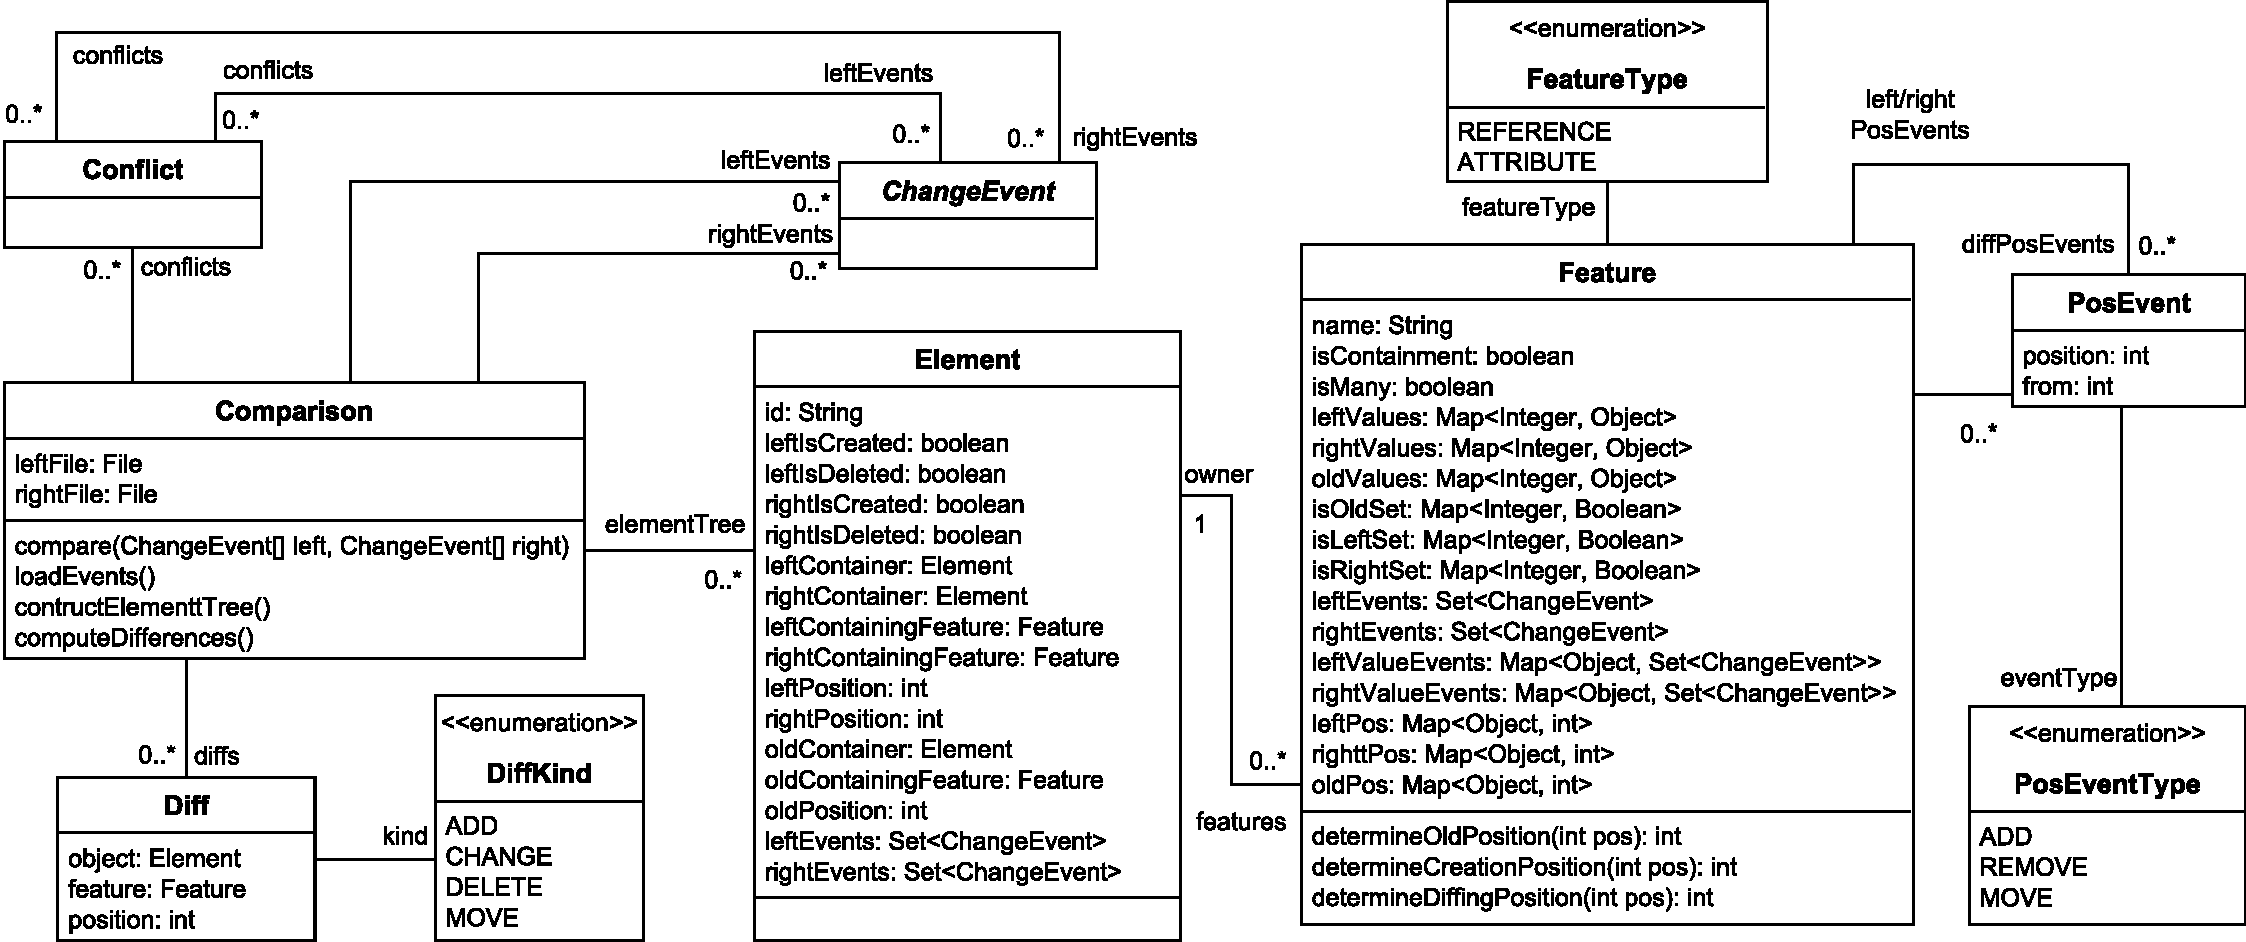
\includegraphics[width=\linewidth]{TreeClassDiagram}
    \caption{A class diagram showing the core components of the change-based approach to speed up model differencing.}
    \label{fig:approach_class_diagram}
  \end{figure}
\end{landscape}

\subsection{Element Tree}
\label{sec:tree_construction}
An element tree is a representation of the changes of model elements in the source and reference models. It contains detailed information about elements and their properties. It contains similar information to that captured in change lists in state-based model persistence, but also provides more information about the changes. For example, the element tree can keep track of a feature's old value and element/value's indexes inside multi-valued properties. The element tree only contains the partial states of affected elements of the original, left, and right models as depicted in Figures \ref{fig:left_element_tree_diagram} and \ref{fig:right_element_tree_diagram}.

To better understand the construction of an element tree from change events, we use the following running example using both change events in the Listings \ref{lst:cbp_left} and \ref{lst:cbp_right}. We start from the left change events. 

\subsubsection{Left Side}\label{sec:left_side}
In the first change event in Listing \ref{lst:cbp_left} at line \ref{line:cbp_left_30}, the change event is a \textsf{session} event. It marks that the all the following change events until the final line or next \textsf{session} event are persisted in one batch when saving. At line \ref{line:cbp_left_31}, we can identify that Bob created a \textsf{Generalization} with id \textsf{leftGen}. Thus, in \textsf{elementTree}, an element with id \textsf{leftGen} is also created. To mark that an element is newly created in the session, we put a '+' sign at the left lower box of element \textsf{leftGen} in Figure \ref{fig:left_element_tree_diagram}.

\begin{figure}[ht]
  \centering
  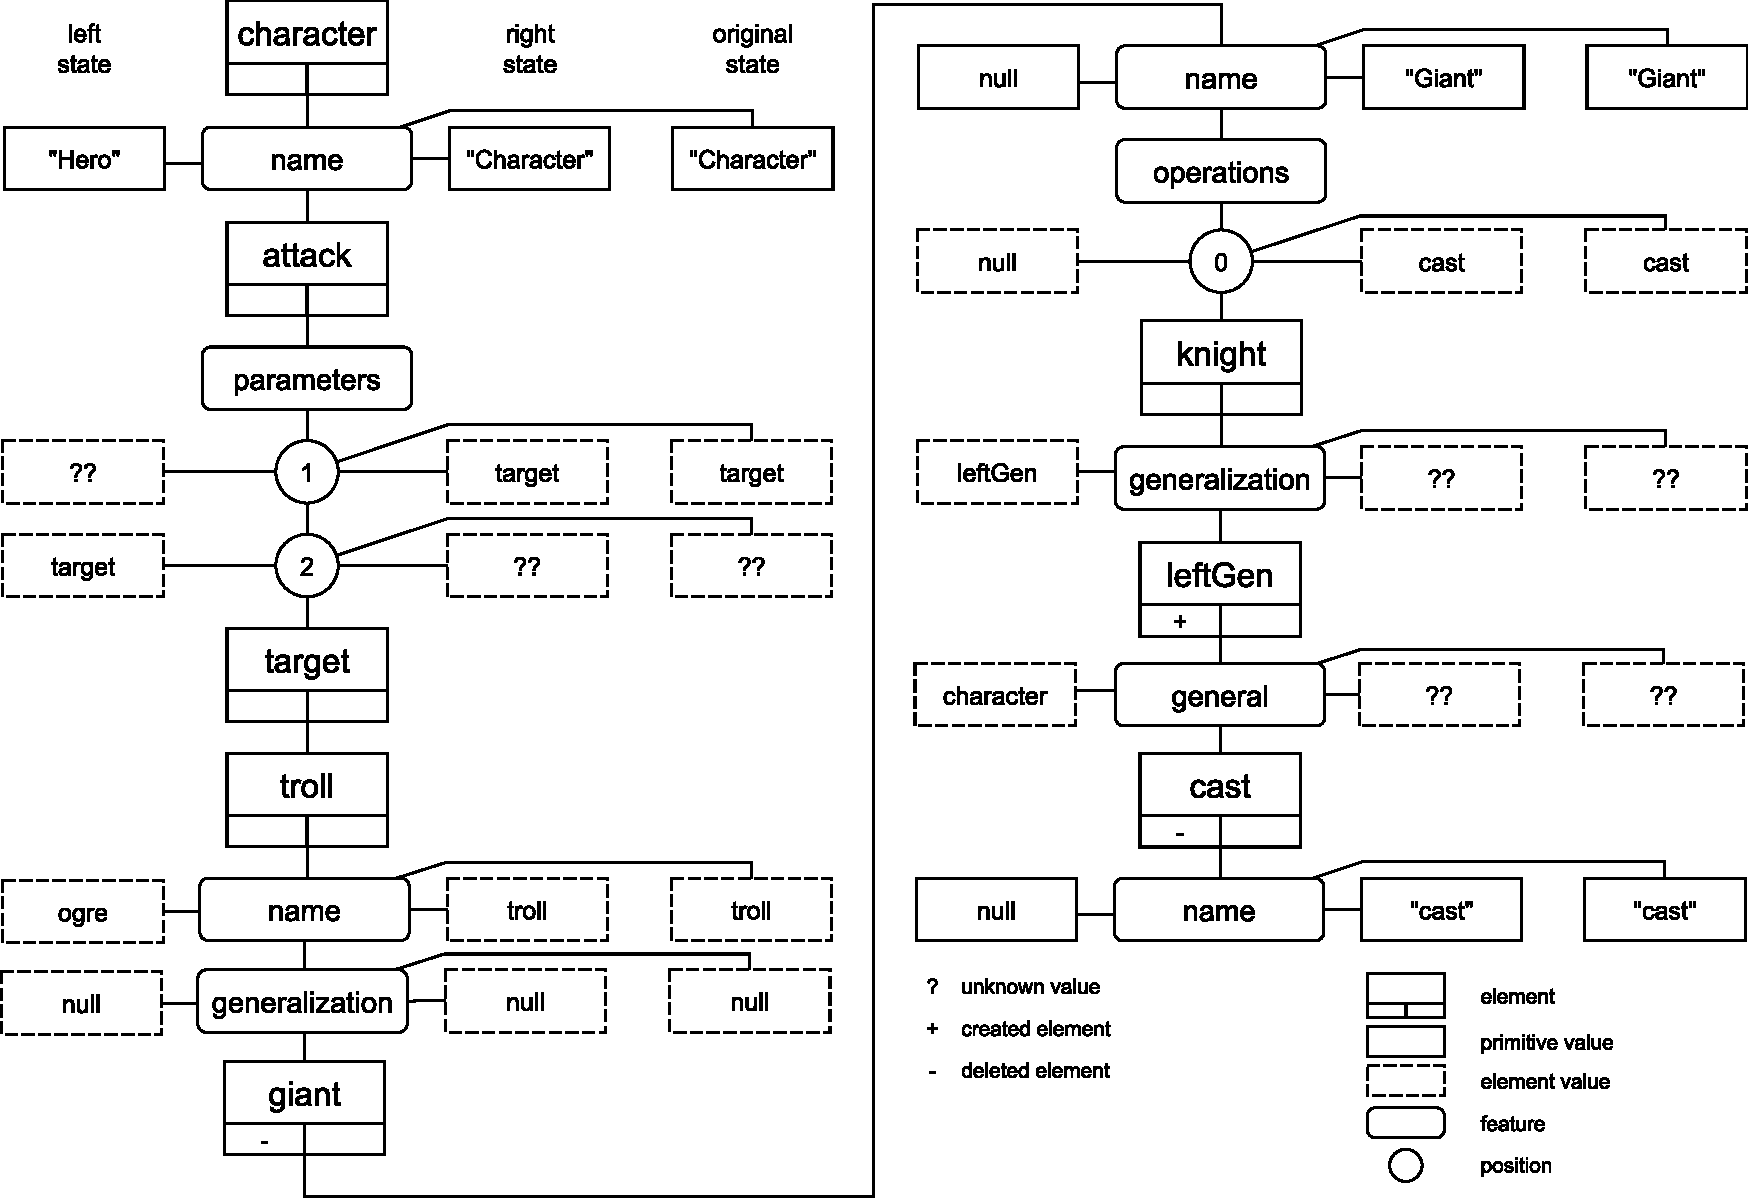
\includegraphics[width=\linewidth]{element_tree_game_left}
  \caption{An element tree constructed using information contained in CBPs in Listing \ref{lst:cbp_left} (all left change events only).}
  \label{fig:left_element_tree_diagram}
\end{figure} 

At line \ref{line:cbp_left_32}, the feature \textsf{general} of \textsf{leftGen} is set to \textsf{character}. From the change event, we can recognise that \textsf{character} has been existed since the previous version since it has never been created in the current editing session. Thus, we create an element with id \textsf{character} as well as the feature \textsf{general} of \textsf{leftGen} and put them in \textsf{elementTree} and then set the value of \textsf{general} to \textsf{character} on the left side. We also do the same routine to \textsf{troll} and \textsf{generalization} at line \ref{line:cbp_left_33}, adding element \textsf{troll} and feature \textsf{generalization} to \textsf{elementTree} and set the value of feature \textsf{generalization} to \textsf{leftGen} on the left side of the \textsf{elementTree}. 

Change event at line \ref{line:cbp_left_34}, change \textsf{character}'s \textsf{name} from ``Character'' to ``Hero''. From the change event, we can identify that \textsf{character} has been existed before. Thus, we create element \textsf{character} and feature \textsf{name} into \textsf{elementTree}. We also set the value of \textsf{name} to ``Hero'' on the left side. Since this set change event is the first event for \textsf{character}'s \textsf{name}, we can infer that original value of \textsf{name} is ``Character''. Thus, we set \textsf{name}'s value to ``Character'' on the original side. The value of \textsf{name} on the right side is also set to ``Character'' but will be modified later once we process the right change events (Alice's change events) if there is any change event that affects it. The same routine is also applied when we process the change event at line \ref{line:cbp_left_43} later.

Lines \ref{line:cbp_left_35} and \ref{line:cbp_left_36} are the changes events of  composite move event \textsf{l1}. Element \textsf{leftGen} is removed (unset) from \textsf{troll}'s \textsf{generalization} and then is assigned (set) to \textsf{knight}'s \textsf{generalization}. From these change events, we can identify that element \textsf{knight} also already existed since the original version. Thus, we add it into \textsf{elementTree} together with its  \textsf{generalization} feature. Element \textsf{troll} and its  \textsf{generalization} feature are not added into \textsf{elementTree} any more since they were already added when processing line \ref{line:cbp_left_33}. In \textsf{elementTree}, we set \textsf{troll}'s \textsf{generalization} to null since element \textsf{leftGen} is moved to \textsf{knight}'s \textsf{generalization}.

At line \ref{line:cbp_left_37}, \textsf{target} is moved from index 1 to 2 in \textsf{attack}'s \textsf{parameters}. From the change event, we can identify that there has been element \textsf{target} contained in \textsf{attack}'s \textsf{parameters} at index 1 since the original version. Thus, we put element \textsf{target} and element \textsf{attack} and its \textsf{parameters} feature into \textsf{elementTree}. We also create a map on the left side with a key `2' and a value that points to element \textsf{target} for feature \textsf{parameters}, indicating \textsf{target} is at index 2 in the left version. Since it is the first change event that moves \textsf{target}, we can decide that \textsf{target} is at index 1 in the original version. Thus, we create another map on the original side a map on the left side with a key `1' and a value that also points to \textsf{target}. We also perform this routine to the right side of feature \textsf{parameters}, creating a map with a key `1' and a value that also points to \textsf{target}. It will be modified later once we process the right change events (Alice's change events) if there is any change event that affects the index of \textsf{target}.

Lines \ref{line:cbp_left_38} to \ref{line:cbp_left_42} are the change events of  composite delete event \textsf{l2}; a deletion of element \textsf{giant}. 
A deletion of an element unsets all the features of the elements and its sub elements, removes the sub elements from their containers, and deletes the sub elements and the element from the model. 
As can be noticed,  at line \ref{line:cbp_left_38}, the value of \textsf{cast}'s \textsf{name}  is unset from ``cast'' to null. From the change event, we know that cast has been existed since the original version. Thus, we add element \textsf{cast} and its feature \textsf{name} to \textsf{elementTree} and set its value null on the left side and ``cast'' on the origin and right sides. 

At line \ref{line:cbp_left_39}, \textsf{cast} is removed from \textsf{giant}'s \textsf{operations} at index 0. From it, we can identify that \textsf{giant} and its feature \textsf{operations} exists, and \textsf{cast} is contained in \textsf{giant}'s \textsf{operations} at index 0 in the original version. Thus, we create element \textsf{giant} and its feature \textsf{operations} in \textsf{elementTree}. Three maps also are created in \textsf{operations} for the three sides. Each map contains a key `0', indicating index, and a value that points to element \textsf{cast} except on the left side the value is null since \textsf{cast} is removed from \textsf{giant}'s \textsf{operations}. The deletion of \textsf{cast} at line \ref{line:cbp_left_40} marks \textsf{cast} in \textsf{elementTree} with `-' sign on the left side indicating that the element is deleted from the model in the left version.

Change event at line \ref{line:cbp_left_41} is similar to change event at line At line \ref{line:cbp_left_38} except that it is applied to \textsf{giant}'s \textsf{name}. Since \textsf{giant} has existed in \textsf{elementTree}, only the feature \textsf{name} is added. Its value is set to null on the left side and ``Giant'' on the origin and right sides. The deletion of \textsf{giant} at line \ref{line:cbp_left_42} marks \textsf{giant} in \textsf{elementTree} with `-' sign indicating that the element is deleted from the model in the left version.

Figure \ref{fig:left_element_tree_diagram} illustrates the state of the \textsf{elementTree} after all left change events have been processed. As can be seen, the \textsf{elementTree} exhibits the partial states of the original, left, and right models at once. 

\subsubsection{Right Side}\label{sec:right_side}
In Listing \ref{lst:cbp_right}, similar to processing the left change events, the processing of the right change events (Alice's version) starts with processing the session event at line \ref{line:cbp_right_30}. At line \ref{line:cbp_right_31}, \textsf{target} is moved from index 1 to 0 in \textsf{attack}'s \textsf{parameters}. Since the index of \textsf{target} is already determined when processing the change event, we only determine the index of \textsf{target} on the right side. We unset the value of key `1' on the right side to null and create a new key `0' that maps its value to \textsf{target}.

Composite move event \textsf{r1} at lines \ref{line:cbp_right_32} and \ref{line:cbp_right_33} moves \textsf{smash} from \textsf{knight}'s \textsf{operations} to \textsf{giant}'s \textsf{operations}. From this move event, we can identify \textsf{smash} is no longer in \textsf{knight}'s \textsf{operations} but contained in \textsf{giant}'s \textsf{operations} on the right side. Element \textsf{smash} has never existed in \textsf{elementTree}. So, we create and add \textsf{smash} to \textsf{knight}'s \textsf{operations} at index 0 on the origin side and to \textsf{giant}'s \textsf{operations} at index 0 on the right side. Since \textsf{smash} is not modified on the left side and no other change events applied to \textsf{knight}'s \textsf{operations}, we can determine that \textsf{smash} is at index 0 in \textsf{giant}'s \textsf{operations} on the left side.

Lines \ref{line:cbp_right_34} to \ref{line:cbp_right_35} are change events that constitute composite move event \textsf{r2}.  It  moves \textsf{cast} from \textsf{giant}'s \textsf{operations} to \textsf{mage}'s \textsf{operations}. From this move event, we can identify \textsf{cast} is no longer in  \textsf{giant}'s \textsf{operations} but now exists in \textsf{mage}'s \textsf{operations} on the right side. Element \textsf{mage} and its feature \textsf{operations} have never existed in \textsf{elementTree}. So, we create and add them to \textsf{elementTree} and add \textsf{cast} to \textsf{mage}'s \textsf{operations} on the right side.

At line \ref{line:cbp_right_36}, we can identify that Alice created a \textsf{Generalization} with id \textsf{rightGen}. Thus, in \textsf{elementTree}, an element with id \textsf{rightGen} is also created. Since it has just been created in the active session, the element is marked with '+' sign in \textsf{elementTree} on the right side. At line \ref{line:cbp_right_37}, we can also identify that feature \textsf{general} should be added to \textsf{rightGen} in \textsf{elementTree} and the value is set to \textsf{character} on the right side. We also set \textsf{mage}'s \textsf{operations} to \textsf{rightGen} on the right side of  \textsf{elementTree} according to the change event at line \ref{line:cbp_right_38}. 

Change event at line \ref{line:cbp_right_39}, change \textsf{character}'s \textsf{name} from ``Character'' to ``Hero''. Since \textsf{character} and its feature \textsf{name} already exists in \textsf{elementTree}, we only set \textsf{name}'s value to ``Hero'' on the right side; the original value has already been assigned when processing left change events. We apply the same routine when processing the change event at line \ref{line:cbp_right_42} later.

\begin{figure}[ht]
  \centering
  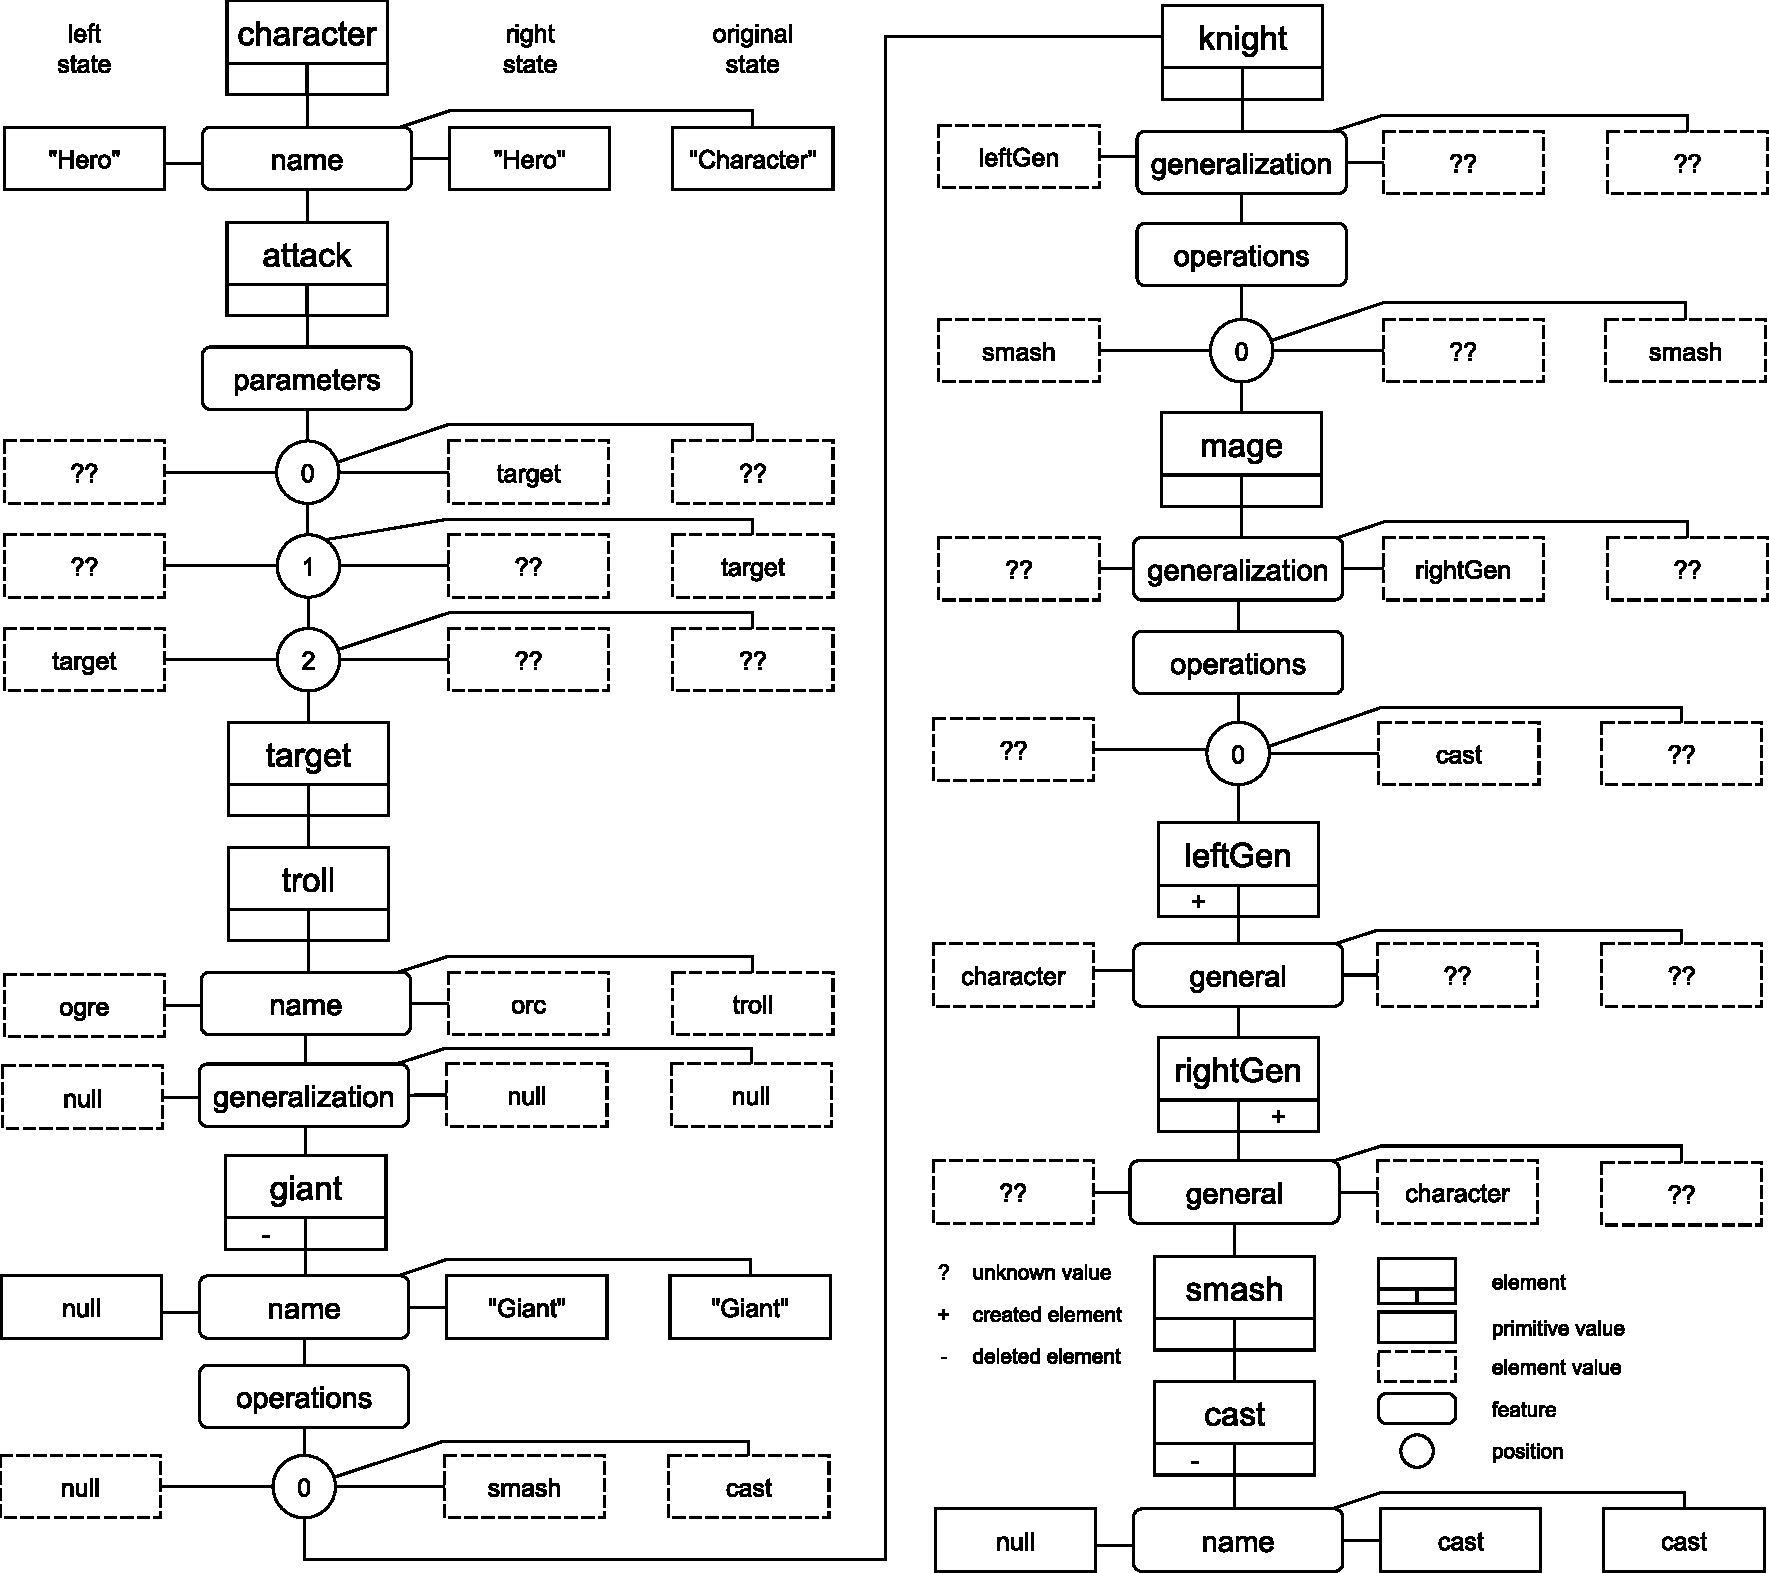
\includegraphics[width=\linewidth]{element_tree_game_right}
  \caption{An element tree constructed using information contained in CBPs in Listings \ref{lst:cbp_left} and \ref{lst:cbp_right} (all left and right change events).}
  \label{fig:right_element_tree_diagram}
\end{figure} 

Composite move event \textsf{r3} at lines \ref{line:cbp_right_40} and \ref{line:cbp_right_41} moves \textsf{rightGen} from \textsf{troll}'s \textsf{generalization} to \textsf{mage}'s \textsf{generalization}. From this move event, on the right side, we can identify \textsf{rightGen} is no longer in \textsf{troll}'s \textsf{generalization} but exists in \textsf{mage}'s \textsf{generalization}. Since it's the first \textsf{mage}'s \textsf{generalization} is modified, we create and add the feature to \textsf{mage} in \textsf{elementTree}. On the right side of \textsf{elementTree}, we unset \textsf{troll}'s \textsf{generalization} to null and assign \textsf{rightGen} to \textsf{mage}'s \textsf{generalization}.

Figure \ref{fig:right_element_tree_diagram} exhibits the state of the \textsf{elementTree} after both sides' change events have been processed.

\begin{figure}
    \centering
    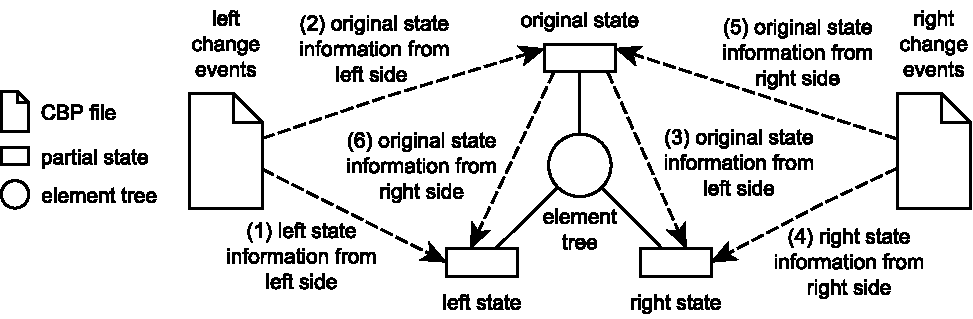
\includegraphics[width=\linewidth]{TreeConstruction}
    \caption{Steps in Element Tree construction.}
    \label{fig:tree_construction}
\end{figure} 

\subsubsection{Construction Procedure}\label{sec:construction_procedure}
The construction of \textsf{elementTree} that has been explained follows the steps shown in Figure \ref{fig:tree_construction}. First, the partial
state $S_{L}$ of the left model in the \textsf{elementTree} is constructed based on the information retrieved from the left change events (step 1). We denote this information as $I_{LL}$. We can also construct the partial 
state $S_{O}$ of the original model using the information related to the original state contained in the left change events $I_{OL}$ (step 2). The information $I_{OL}$ allows us to construct the initial partial 
state $S_{R}$ of the right model 
(step 3). Similarly, using the information from the right change events $I_{RR}$, we update the partial right state $S_{R}$ that has been initialised before using the information $I_{OL}$ (step 4), implying that $I_{OL} \cup I_{RR} \rightarrow S_{R}$. Also, information related to the state of the original model from the right change events $I_{OR}$ is used to update the original state  (step 5). Thus, we have a partial state of the original model constructed using information from both left and right sides, $I_{OL} \cup I_{OR} \rightarrow S_{O}$. Finally, we also use the information $I_{OR}$ to update the partial state of the left model (step 6), implying that $I_{LL} \cup I_{OR} \rightarrow S_{L}$.  

Algorithm \ref{alg:element_tree} describes the steps presented in Figure \ref{fig:tree_construction} in a generic fashion. It iterates through all of a model's change events and uses the information contained in them to construct the relevant partial state. The selection of side, left or right change events, that are executed first depends on the \textsf{Side} enumeration value -- \textsf{left} or \textsf{right} -- passed through the parameter \textsf{side} (the second input parameter). In our implementation, we process the left side first by default. The algorithm also receives an input of the change events \textsf{events} that are to be iterated and the element tree \textsf{elementTree} that has been instantiated before, and then returns the \textsf{elementTree} as output after updating it.

For each \textsf{event} in the \textsf{events}, we collect information needed to build up \textsf{elementTree}  (lines 3-9), such as \textsf{targetElement}, \textsf{feature}, \textsf{value}, \textsf{previousValue}, \textsf{index}, and \textsf{previousIndex}. The \textsf{targetElement} is the element modified by a change event (e.g., \textsf{character} and \textsf{giant} in Listing \ref{lst:cbp_left}). This \textsf{targetElement} -- an instance of class Element in Figure \ref{fig:approach_class_diagram} -- is retrieved from the \textsf{elementTree} if it already exists. Otherwise, a new element is created and added to the \textsf{elementTree} (line 3). In this step we also set the flags \textsf{*IsCreated} and \textsf{*IsDeleted} of the element in Figure \ref{fig:approach_class_diagram}. For example, if the type of the event is \textsf{create} then \textsf{*IsCreated} is set to \textsf{true}. The \textsf{feature} -- an instance of class Feature in Figure \ref{fig:approach_class_diagram} -- represents the target element's feature (e.g., \textsf{name} and \textsf{operations} in Listing \ref{lst:cbp_right}) modified by a change event. It is retrieved from the \textsf{targetElement}'s feature list, and a new one is created and added to the \textsf{targetElement}'s feature list if the feature does exist (line 5). 

\IncMargin{1.5em}
\begin{algorithm}[H]
    \begin{footnotesize}
        \SetKwInOut{Input}{input} 
        \SetKwInOut{Output}{output}
        \Input{a list of ChangeEvent $events$}
        \Input{an enumeration of Side $side$}
        \Input{an instance of ElementTree $elementTree$}
        \Output{an instance of ElementTree $elementTree$}
        \SetKwBlock{Beginn}{beginn}{ende}
        \Begin{
            \ForEach{$event$ in $events$}{
                $targetElement$ $\leftarrow$ getOrCreateNewTargetElement($event$, $elementTree$)\;
                $feature$ $\leftarrow$ getOrCreateNewFeature($event$, $targetElement$)\;
                $value$ $\leftarrow$ getValue($event$)\;
                $previousValue$ $\leftarrow$ getPreviousValue($event$)\;
                $index$ $\leftarrow$ getIndex($event$)\;
                $previousIndex$ $\leftarrow$ getPreviousIndex($event$)\;
                $featureEventList$ $\leftarrow$ getFeatureEventList($feature$, $side$)\;
                
                \BlankLine
                \tcp{put all values to their proper indexes}
                updateTree($targetElement$, $feature$, $value$, $index$, $side$)\;
                $oldIndexes$ $\leftarrow$ calculateOldIndex($featureEventList$, $previousIndex$, $side$)\;
                \If{\Not isCreated($value$, $side$) \AndA \Not isOldValueSet($feature$, $previousValue$, $previousIndex$, $side$)} {
                    setOldValue($feature$, $previousValue$, $oldIndex$, $side$)\;
                    $oppositeFeatureEventList$ $\leftarrow$ getOppositeFeatureEventList($feature$, $side$)\;
                    $oppositeIndex$ $\leftarrow$ calculateOppositeIndex($oppositeFeatureEventList$, $oldIndex$, $side$)\;
                    \If{\Not isDeleted($value$, $side$) \AndA \Not isOppositeSideValueSet($feature$, $value$, $oppositeIndex$, $side$)} {
                        setOppositeSideValue($feature$, $value$, $oppositeIndex$, $side$)\;
                    }
                }   
                
                addEventToFeatureEventList($event$, $featureEventList$)\;
                
            }
            \Return{$elementTree$}\;
        }
    \end{footnotesize}
    \caption{Algorithm to construct an element tree from events.}
    \label{alg:element_tree}
\end{algorithm}
\DecMargin{1.5em}

The \textsf{value} is the value assigned to the feature in a change event (line 5, Algorithm \ref{alg:element_tree}). The \textsf{value} can be the type of \textsf{Element} (e.g., element \textsf{leftGen} line \ref{line:cbp_left_36} in Listing \ref{lst:cbp_left}) or primitive (e.g., the string ``Hero'' at line \ref{line:cbp_left_34} in the Listing \ref{lst:cbp_left}). The \textsf{previousValue} represents the previous value of the modified feature (line 6, Algorithm \ref{alg:element_tree}). The \textsf{previousValue} is not defined if no previous value has been assigned. For \textsf{value} and \textsf{previousValue} with type \textsf{Element}, the elements that they represent are retrieved from the \textsf{elementTree}, and if they do not exist, new instances are created. If the type is primitive, the value is treated as it is. Not every change event has a \textsf{value}, particularly events with type \textsf{create} 
or \textsf{delete} which only modify a target element not the element's feature.

The \textsf{index} is the index assigned by a change event to a value in a feature, while \textsf{previousIndex} is the previous index of the value (lines 7-8, Algorithm \ref{alg:element_tree}). In one change event, we can get both \textsf{index} and \textsf{previousIndex} or only one of them depending on the type of the change event. For example, we can obtain that the \textsf{index} of \textsf{cast} is 0 (line \ref{line:cbp_right_35} in Listing \ref{lst:cbp_right}) as the change event type is \textsf{add}. In a \textsf{remove} change event, we can only get the \textsf{previousIndex} of \textsf{cast}, that is 1 (line \ref{line:cbp_right_35} in Listing \ref{lst:cbp_right}), as the element does not exist anymore in the left model. We can obtain both of them only in a \textsf{move} change event as an element is moved from a previous index to a new one (line \ref{line:cbp_right_31} in Listing \ref{lst:cbp_right}). For a single-valued feature, the \textsf{index} and \textsf{previousIndex} are always 0 as the feature can only contain a single value. 

At line 9, we retrieve the \textsf{featureEventList} from the \textsf{feature} to be added later with the current \textsf{event} (line 19). The \textsf{featureEventList} is a list -- a history -- of change events that have been processed that are specific to the \textsf{feature} on the selected \textsf{side}. Using the obtained \textsf{targetElement}, \textsf{feature}, \textsf{value}, and \textsf{index}, the process then updates the state of the \textsf{elementTree} on the selected \textsf{side} (line 10). After that, it calculates back the original index of a value using the \textsf{featureEventList} and \textsf{previousIndex} (line 11). If the value at \textsf{oldIndex} in the \textsf{feature} has not been set, then the algorithm sets the \textsf{feature} with the \textsf{previousValue} at the \textsf{oldIndex} in the partial state of the original model (lines 12-13). At lines 14-18, the algorithm also does the same thing to the opposite side -- if the current \textsf{side} is \textsf{left} then it is \textsf{right}.  

\subsection{Diff Computation}
\label{sec:diff_computation}
Using the \textsf{elementTree} presented in Figure \ref{fig:right_element_tree_diagram}, we can determine the difference between the left and right models without having to compare all their elements and features. After the \textsf{elementTree} has been constructed, we iterate through elements and features of the \textsf{elementTree} and use the flags, containers, containing features, and indexes on both sides of each element and value to identify differences between both left and right models. We follow the steps in Algorithm \ref{alg:diff_calculation}. The algorithm visits each element and every index of each feature (lines 3-5). At every index, it retrieves the \textsf{leftValue} and \textsf{rightValue} (lines 5-7), passing these, together with the \textsf{element}, \textsf{feature}, and \textsf{index} to a function \textsf{identifyDiffUsingRules} (line 8). The function identifies differences using a set of pre-defined rules which determines differences \textsf{diffs} based on the states of flags of an element, flags and attributes of the element's feature, values of the feature, and indexes of the values. The obtained \textsf{diffs} are then added to the overall list of differences \textsf{diffList} which is output (line 8-9, 13). 

\IncMargin{1.5em}
\begin{algorithm}[H]
    \begin{footnotesize}
        \SetKwInOut{Input}{input}
        \SetKwInOut{Output}{output}
        \Input{an instance of ElementTree $elementTree$}
        \Begin{
            $diffList$ $\leftarrow$  DiffList()\;
            \ForEach{$element$ \In $elementTree$}{
                \ForEach{$feature$ \In getFeatures($element$)}{
                    \ForEach{$index$ \In getIndexes($feature$)}{
                        $leftValue$ $\leftarrow$ getLeftValue($feature$, $index$)\;
                        $rightValue$ $\leftarrow$ getRightValue($feature$, $index$)\;
                        \BlankLine
                        \tcp{rules starts from here}
                        $diffs$ $\leftarrow$ identifyDiffUsingRules($element$, $feature$, $leftValue$, $rightValue$, $index$)\;
                        addToDiffList($diffs$,$diffList$)\;
                    }
                }
            }
            \Return{$diffList$}\;
        }
    \end{footnotesize}
    \caption{Algorithm to determine differences.}
    \label{alg:diff_calculation}
\end{algorithm}
\DecMargin{1.5em}

We illustrate the principles and use of rules by discussing the rules used to identify differences in the running example, which can be found in Algorithm \ref{alg:diff_rules}. The algorithm is the breakdown of the function \textsf{identifyDiffUsingRules} in Algorithm \ref{alg:diff_calculation}. As previously stated, it is important to remember that we use the left model as a reference which means the differences are presented as changes that transform the right model to become equal to the left model. 

The first rule (Rule 1) in Algorithm \ref{alg:diff_rules} is to identify changes in single-valued attributes. A feature has to be of type \textsf{attribute}, both side values have to be different, and the element should have not been created or deleted in both models. The second rule (Rule 2) identifies whether an element is in a different location in both models. The element must not have been deleted and must exist from the previous version -- the original model. Also, its containers, containing features, or indexes of the element have to be different on both sides.The third rule (Rule 3) identifies the deletion of an element. If an element in the left model is not created but exists in the model, it means that the element has been there from the previous version -- the original model. This also means that the element also exists in the right model, unless it has been deleted. Thus, in order to make the right model equal to the left model, the element has to be deleted also in the right model. 

Similar to Rule 3, the fourth rule (Rule 4) in Algorithm \ref{alg:diff_rules_2} also identifies the deletion of an element except that it identify an element that only created in the right model and it has not been deleted. Thus, in order to make the right model equal to the left model, the element has to be deleted from the right model. The fifth rule (Rule 5) identifies the need for an addition of an element. If an element is created in the left model and has not been deleted, it means that the element should be added also to the right model to make both models equal.

\IncMargin{1.5em}
\begin{algorithm}[]
    \begin{footnotesize}
        \SetKwInOut{Input}{input}
        \SetKwInOut{Output}{output}
        \Input{an Element $element$, a Feature $feature$, a variable $leftValue$, a variable $rightValue$, an Integer $index$}
        \Output{a List of Diff $diffs$}
        $diffs$ $\leftarrow$ createDiffList()\;
        \tcp{...}
        \tcp{Rule 1: a rule to determine a change of a single-valued attribute}
        \If{getType($feature$) \Is Attribute \AndA isSingleValued($feature$) \AndA leftValue <> rightValue \AndA \Not leftIsCreated($element$) \AndA \Not leftIsDeleted($element$) \AndA \Not  rightIsCreated($element$) \AndA \Not rightIsDeleted($element$)}{
            $diff$ $\leftarrow$ createNewDiff($element$, $element$, $feature$, $feature$, $index$, $index$, $leftValue$, $rightValue$, DifferenceType.CHANGE)\;
            addDiffToDiffList($diff$, $diffs$)\;
        } 
        \tcp{Rule 2: one of rules to determine movement of an element (only for right value, left value has its own rule)}
        \If{getType($feature$) \Is Containment \AndA \Not isNull($rightValue$) \AndA \Not leftIsCreated($rightValue$) \AndA \Not leftIsDeleted($rightValue$) \AndA \Not rightIsCreated($rightValue$) \AndA \Not rightIsDeleted($rightValue$) \AndA (getLeftContainer($rightValue$) <> getRightContainer($rightValue$) \Or getLeftFeature($rightValue$) <> getRightFeature($rightValue$) \Or getLeftIndex($rightValue$) <> getRightIndex($rightValue$))}{
            $diff$ $\leftarrow$ createNewDiff(getLeftContainer($rightValue$), getRightContainer($rightValue$), getLeftFeature($rightValue$), getRightFeature($rightValue$), getLeftIndex($rightValue$), getRightIndex($rightValue$), $rightValue$, $rightValue$, DifferenceType.MOVE)\;
            addDiffToDiffList($diff$, $diffs$)\;
        }
        \tcp{Rule 3: one of rules to determine deletion of an element}
        \If{getType($feature$) \Is Containment \AndA \Not  leftIsCreated($rightValue$) \AndA leftIsDeleted($rightValue$) \AndA \Not rightIsCreated($rightValue$) \AndA \Not rightIsDeleted($rightValue$) }{
            createNewDiff(getLeftContainer($rightValue$), getRightContainer($rightValue$), getLeftFeature($rightValue$), getRightFeature($rightValue$), null, getRightIndex($rightValue$), null, $rightValue$, DifferenceType.DELETE)\;
            addDiffToDiffList($diff$, $diffs$)\;
        }
        \tcp{...}
        \tcp{continue to part 2}
    \end{footnotesize}
    \caption{Some rules to determine differences (part 1).}
    \label{alg:diff_rules}
\end{algorithm}
\DecMargin{1.5em}


\IncMargin{1.5em}
\begin{algorithm}[]
  \begin{footnotesize}
    \tcp{continuation of part 1}
    \tcp{...}
    \tcp{Rule 4: one of rules to determine deletion of an element}
    \If{getType($feature$) \Is Containment \AndA \Not leftIsCreated($rightValue$) \AndA \Not leftIsDeleted($rightValue$) \AndA rightIsCreated($rightValue$) \AndA rightIsDeleted($rightValue$) }{
      createNewDiff(getLeftContainer($rightValue$), getRightContainer($rightValue$), getLeftFeature($rightValue$), getRightFeature($rightValue$), null, getRightIndex(rightValue), null, $rightValue$, DifferenceType.DELETE)\;
      addDiffToDiffList($diff$, $diffs$)\;
    }
    \tcp{Rule : one of rules to determine addition of an element}
    \If{getType($feature$) \Is Containment \AndA leftIsCreated($leftValue$)  \AndA \Not leftIsDeleted($leftValue$) \AndA \Not rightIsCreated($leftValue$) \AndA \Not rightIsDeleted($leftValue$)}{
      $diff$ $\leftarrow$ createNewDiff(getLeftContainer($leftValue$), getRightContainer($leftValue$), getLeftFeature($leftValue$), getRightFeature($leftValue$), getLeftIndex($leftValue$), null, $rightValue$, null, DifferenceType.ADD)\;
      addDiffToDiffList($diff$, $diffs$)\;
    }
    \tcp{...}
    \Return{$diffs$}
  \end{footnotesize}
  \caption{Some rules to determine differences (part 2).}
  \label{alg:diff_rules_2}
\end{algorithm}
\DecMargin{1.5em}

In Figure \ref{fig:right_element_tree_diagram}, when the iteration of \textsf{elementTree}, from element \textsf{character} down to feature \textsf{name} of element \textsf{cast}, reaches index 0 in feature \textsf{parameters} of element \textsf{attack}, we can identify that \textsf{rightValue} has the value element \textsf{target} and the value of  \textsf{leftValue} is unknown. As \textsf{rightValue} is not null and value \textsf{target} exists on both sides -- all its \textsf{*Created} and \textsf{*Deleted} flags are false, and it also has a different index, at 2 in the left state and 0 in the right state. This meets the condition of the second rule.Thus, we can conclude that in order to make the index of element \textsf{target} in the right model equal its index in the left model, element \textsf{target} should be moved from index 0 to 2. Thus, the type of this difference is \textsf{MOVE}. We denote this difference as $dc_{1}$. The same rule is also applied to element \textsf{smash} when the iteration reach index 0 in \textsf{knight}'s \textsf{generalization}. Applying the rule to the element produces difference $dc_{3}$.

When the iteration is at feature \textsf{name} of element \textsf{troll}, we obtain that the type of the feature is a single-valued attribute and both sides of the feature are different in their values. This means that the condition of the first rule is met. Thus, we can conclude that in order to make the left value of the feature equal to the right value, we must override the value ``Orc'' with ``Ogre''; the type of this difference is \textsf{CHANGE}. We denote this difference as $dc_{2}$.

At \textsf{giant}, the element used to exist but has been deleted from the left model (flags \textsf{leftIsCreated} = false, \textsf{leftIsDeleted} = true); it still exists in the right state (flags \textsf{rightIsCreated} = false, \textsf{rightIsDeleted} = false). This condition satisfies the third rule. Therefore, element \textsf{giant} should be deleted from the right model; the type of this difference is \textsf{DELETE}. We denote this difference as $dc_{4}$. The same rule is applied to element \textsf{cast} when the iteration reach the element. Applying the rule to the element produces difference $dc_{6}$.

We can get only one value when the iteration is at index 0 in the element \textsf{knight}'s feature \textsf{generalization}; the \textsf{leftValue} is element \textsf{leftGen}, but the \textsf{rightValue} is unidentified. Thus, we only process the \textsf{leftValue}. Element \textsf{leftGen} is only created in the left model (flags \textsf{leftIsCreated} = true, \textsf{leftIsDeleted} = false, \textsf{rightIsCreated} = false, \textsf{rightIsDeleted} = false). This meets the condition of the fifth rule. Thus, to make element \textsf{leftGen} also exist in the right state, we must add it into element \textsf{knight}'s feature \textsf{generalization} at index 0. Therefore, the type of this difference is \textsf{ADD}. We denote this difference as $dc_{7}$.

When the iteration is at index 0 in the element \textsf{mage}'s feature \textsf{generalization}, We can get only one value; the \textsf{leftValue} is unidentified and the \textsf{rightValue} is element \textsf{rightGen}. Therefore, we only process the \textsf{rightValue}. Element \textsf{rightGen} is only created in the right model (flags \textsf{leftIsCreated} = false, \textsf{leftIsDeleted} = false, \textsf{rightIsCreated} = true, \textsf{rightIsDeleted} = false). This meets the condition of the fourth rule. Thus, to make element \textsf{rightGen} also does not exist in the left state, we must delete it from index 0 in element \textsf{mage}'s feature \textsf{generalization}. Therefore, the type of this difference is \textsf{DELETE}. We denote this difference as $dc_{5}$.

%$ds_{1}$ =  [\textsf{attack}, \textsf{attack}, \textsf{parameters}, \textsf{parameters}, 1, 0, \textsf{gem}, \textsf{gem}, \textsf{MOVE}]\\
%$ds_{2}$ = [\textsf{troll}, \textsf{troll}, \textsf{name}, \textsf{name}, 0, 0, ``Ogre'', ``Orc'', \textsf{CHANGE}]\\
%$ds_{3}$ = [\textsf{knight}, \textsf{giant}, \textsf{operations}, \textsf{operations}, 0, 0, \textsf{smash}, \textsf{smash}, \textsf{MOVE}]\\
%$ds_{4}$ = [\textsf{resource}, \textsf{resource}, \textsf{null}, \textsf{null}, \textsf{null}, 2, \textsf{null}, \textsf{giant}, \textsf{DELETE}]\\
%$ds_{5}$ = [\textsf{mage}, \textsf{mage}, \textsf{generalization}, \textsf{generalization}, \textsf{null}, 0, \textsf{null}, \textsf{rightGen}, \textsf{DELETE}] \\
%$ds_{6}$ = [\textsf{mage}, \textsf{mage}, \textsf{operations}, \textsf{operations}, \textsf{null}, 0, \textsf{null}, \textsf{cast}, \textsf{DELETE}]\\
%$ds_{7}$ = [\textsf{knight}, \textsf{knight}, \textsf{generalization}, \textsf{generalization}, 0, \textsf{null}, \textsf{leftGen}, \textsf{null}, \textsf{ADD}]

Similar to the state-based approach in Section \ref{sec:state-based_model_differencing}, we express identified differences as $dc_{n}$ = [$LeftContainer_n$, $RightContainer_n$, $LeftFeature_n$, $RightFeature_n$, $LeftIndex_n$, $RightIndex_n$, $LeftValue_n$, $RightValue_n$, $Kind_n$]. Thus:

$dc_{1}$ =  [\textsf{attack}, \textsf{attack}, \textsf{parameters}, \textsf{parameters}, 2, 0, \textsf{target}, \textsf{target}, \textsf{MOVE}]\\
$dc_{2}$ = [\textsf{troll}, \textsf{troll}, \textsf{name}, \textsf{name}, 0, 0, ``Ogre'', ``Orc'', \textsf{CHANGE}]\\
$dc_{3}$ = [\textsf{knight}, \textsf{giant}, \textsf{operations}, \textsf{operations}, 0, 0, \textsf{smash}, \textsf{smash}, \textsf{MOVE}]\\
$dc_{4}$ = [\textsf{resource}, \textsf{resource}, \textsf{null}, \textsf{null}, \textsf{null}, 2, \textsf{null}, \textsf{giant}, \textsf{DELETE}]\\
$dc_{5}$ = [\textsf{mage}, \textsf{mage}, \textsf{generalization}, \textsf{generalization}, \textsf{null}, 0, \textsf{null}, \textsf{rightGen}, \textsf{DELETE}] \\
$dc_{6}$ = [\textsf{mage}, \textsf{mage}, \textsf{operations}, \textsf{operations}, \textsf{null}, 0, \textsf{null}, \textsf{cast}, \textsf{DELETE}]\\
$dc_{7}$ = [\textsf{knight}, \textsf{knight}, \textsf{generalization}, \textsf{generalization}, 0, \textsf{null}, \textsf{leftGen}, \textsf{null}, \textsf{ADD}]

This change-based approach might produce differences that are distinct from differences identified using state-based approach. This can be seen between by comparing $ds_{1}$ and $dc_{1}$ ($ds_{1}$ $\neq$ $dc_{1}$,  [\textsf{attack}, \textsf{attack}, \textsf{parameters}, \textsf{parameters}, 0, 1, \textsf{gem}, \textsf{gem}, \textsf{MOVE}] $\neq$ [\textsf{attack}, \textsf{attack}, \textsf{parameters}, \textsf{parameters}, 2, 0, \textsf{target}, \textsf{target}, \textsf{MOVE}]). State-based approach identifies element \textsf{gem} as the element that should be moved to index 0 to resolve difference in \textsf{attack}'s \textsf{parameters} ($ds_{4}$), while in the change-based approach, the difference is attributed to element \textsf{target} ($dc_{4}$). However, in both approaches, if we resolve their differences by performing all-left-to-right merging  -- making the right model equal to the left model, both approaches produce two models that are equivalent. In this way, we can check the correctness of the identified differences produced by the change-based approach.

\vspace{-10pt}
\section{Evaluation}
\label{sec:evaluation_6}
In this section, the method that was employed to evaluate the proposed change-based model differencing approach as well as the evaluation results are presented and discussed. 

\subsection{Method}
\label{sec:method}
In order to assess the performance benefits of the change-based approach in terms of model differencing, we have evaluated it against a mature and widely-used state-based comparison tool (EMF Compare \cite{emfcompare2018developer,eclipse2017compare}). Since there are no manually developed, large models persisted in our change-based format yet, the dataset for our experiments was constructed from a large model reverse-engineered from the Eclipse Epsilon project \cite{eclipse2018epsilongit,eclipse2017epsilon}. This model conforms to the Java metamodel \cite{eclipse2018modiscojava} and consists of more than 1.6 million elements with a size of 224 MBs when persisted in XMI. 

We cloned the original model to produce two new (left and right) models and perform operations (\textsf{add}, \textsf{remove}, \textsf{move}, \textsf{set} with random elements, features, indexes, and values) on both models to create differences. We made 1.1 million artificial changes to each model, generating over 1.1 million events (one operation can generate more than one event, e.g., a \textsf{move} between features generates \textsf{remove} and \textsf{add} events). Events generated by the changes were persisted in our change-based format (to be used later in change-based model differencing). After every 50,000 changes, we made a measurement point. We persisted the last state of the models in state-based format (to be used later in state-based model differencing) and then performed change-based and state-based model differencing and measured their execution time and memory footprint. We created 22 measurement points to capture their trends in one experiment. 

We conducted five experiments. In the first experiment, the ratio of occurrence between \textsf{add}, \textsf{remove}, \textsf{move}, and \textsf{set} changes is set to 1:1:20:40 intuitively in assumption that in a mature model modification -- \textsf{move} and \textsf{set} events -- occurs more frequent than addition and deletion. Since we wanted the change of total elements not to affect our measurement, the number of total elements should be kept constant. For example, it is difficult to tell an increase of time in comparison is caused by an increase in the number of elements or by the number of change events. One way to do this was to exclude \textsf{add} and \textsf{remove} operations. However, excluding both operations made measurement less representative. Thus, we still included both operations but made their probabilities equal so that the number of total elements remain largely unchanged. In the rest of the experiments,
we only performed homogeneous type operations -- isolated from other types -- per experiment (e.g., add-only, move-only operations). In the end, we obtained 5 results of the experiments: mixed, add-only, remove-only, move-only, and set-only measurement results. We did this to asses whether operations of different types have a different impact on model differencing.

\begin{wrapfigure}[13]{r}{0.5\textwidth}
  \vspace{-5pt}
  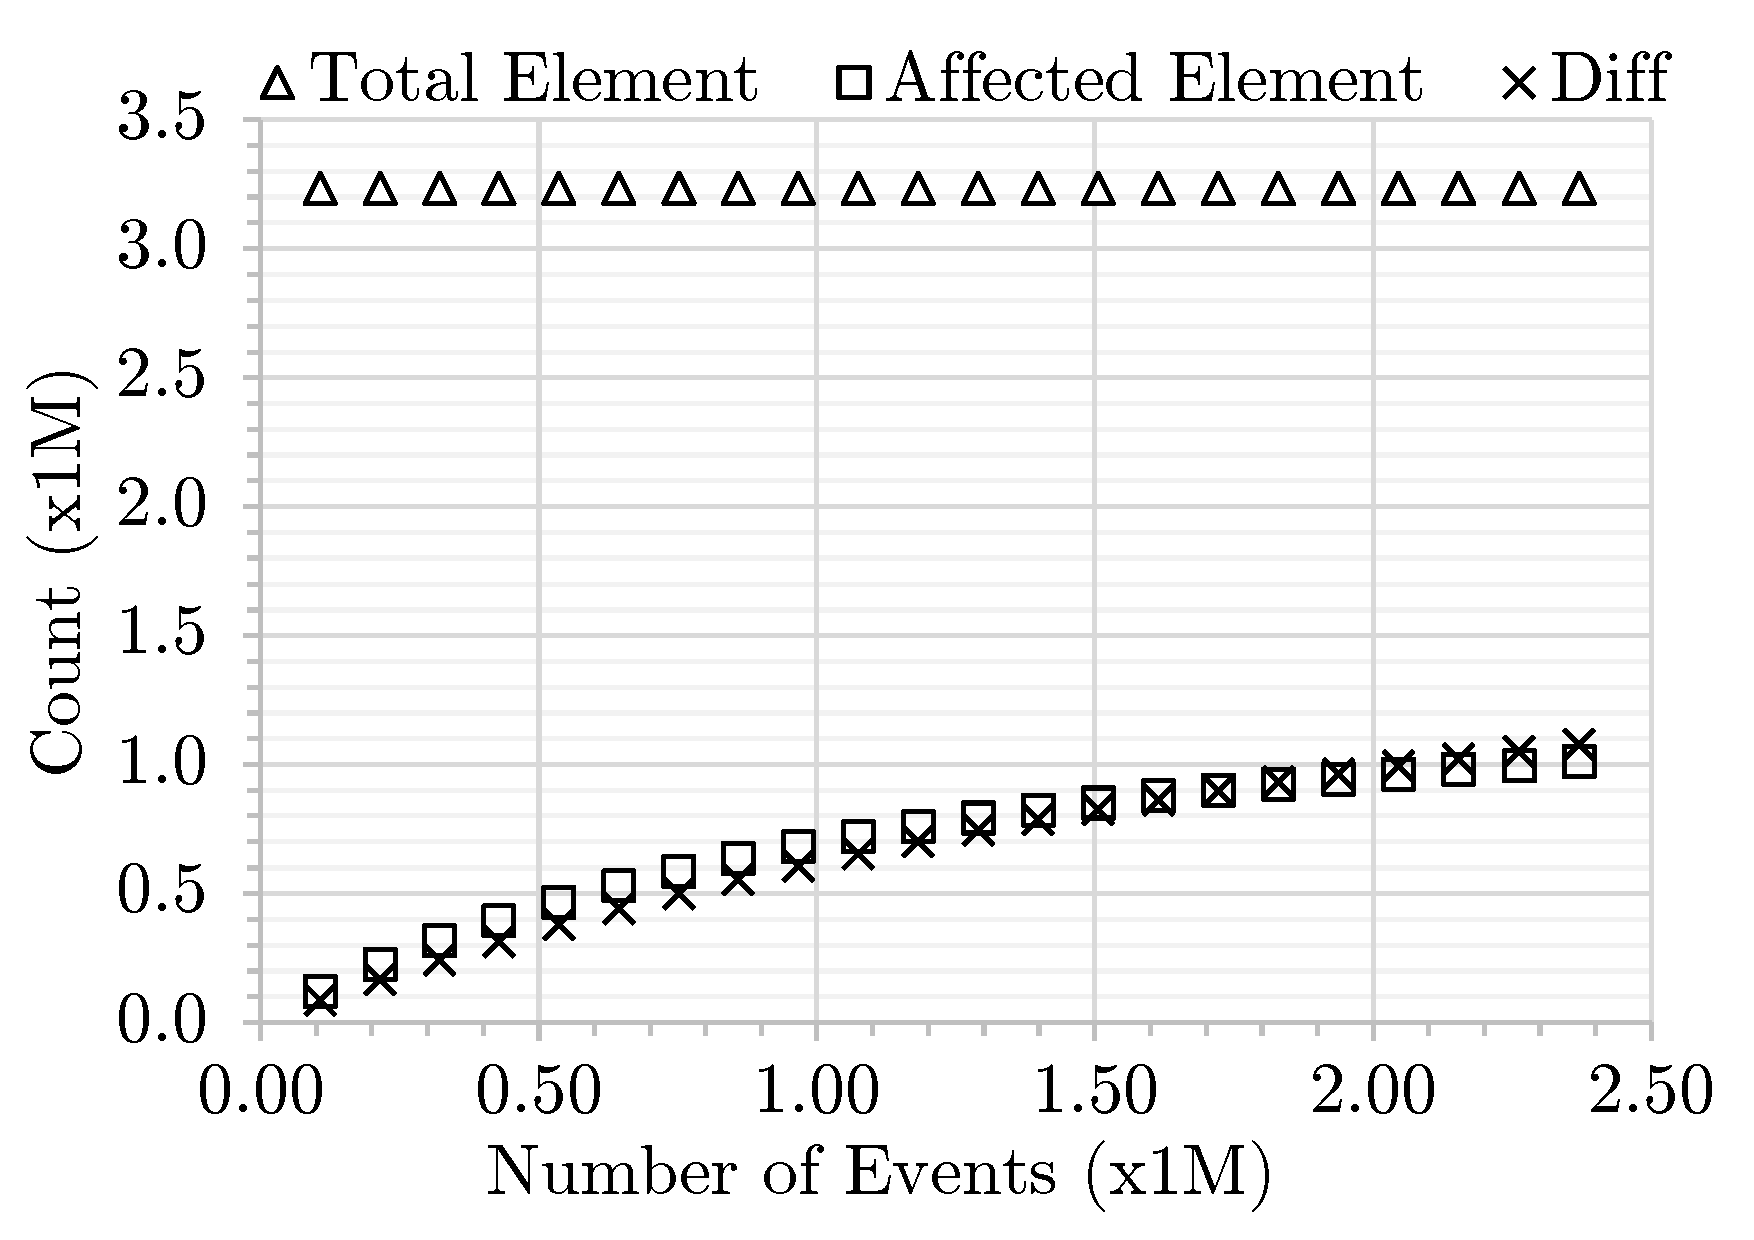
\includegraphics[width=\linewidth]{mixed-count-events}
  \caption{total elements, affected elements, and diffs}
  \label{fig:modification_course}
\end{wrapfigure}

For the change-based approach, the comparison time comprises loading change events, constructing an element tree, and identifying differences. The memory footprint is the space used to hold the change events, element tree, and differences in memory. For the state-based approach, the comparison time comprises matching elements and identifying differences, and the memory footprint is the space required to hold the matches and differences in memory. All measurements were performed on the same machine with the following specification: AMD Opteron(tm) Processor 6386 SE @ 2.8 GHz cache size 2 GBs (64 processors), 528 GBs main memory, Ubuntu 16.04.6 LTS operating system, and Java(TM) SE Runtime Environment (build 1.8.0\_201-b09) with JVM \textsf{InitialHeapSize} 2GBs and \textsf{MaxHeapSize} 32 GBs.

\subsection{Results and Discussion}
\label{sec:results_and_discussion}
In this section, we report on the obtained results in terms of comparison time and memory footprint for the mixed and homogeneous operation experiments. 

\begin{figure}[ht]
  \begin{subfigure}[t]{0.495\linewidth}
    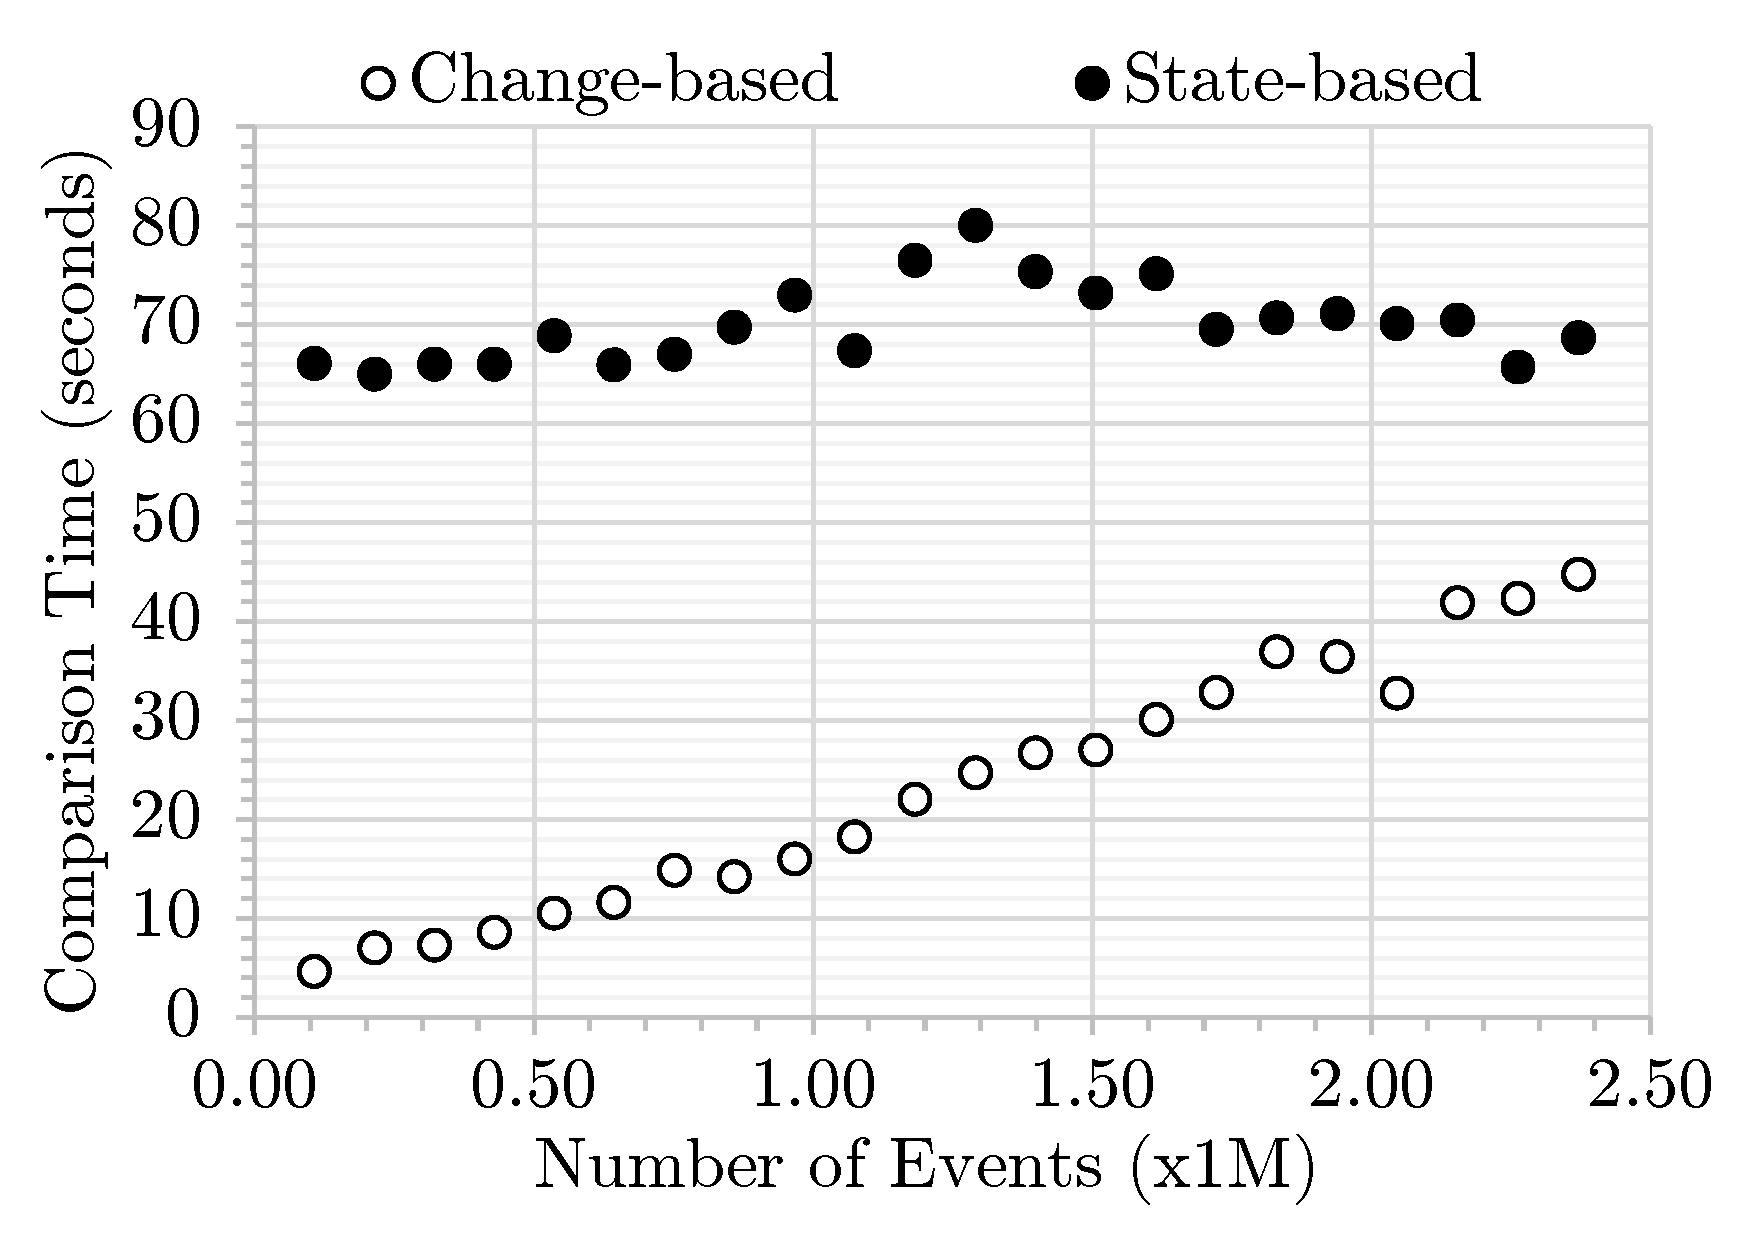
\includegraphics[width=\linewidth]{mixed-time-events}
    \caption{execution time}
    \label{fig:time_diffs}
  \end{subfigure}
  \begin{subfigure}[t]{0.495\linewidth}
    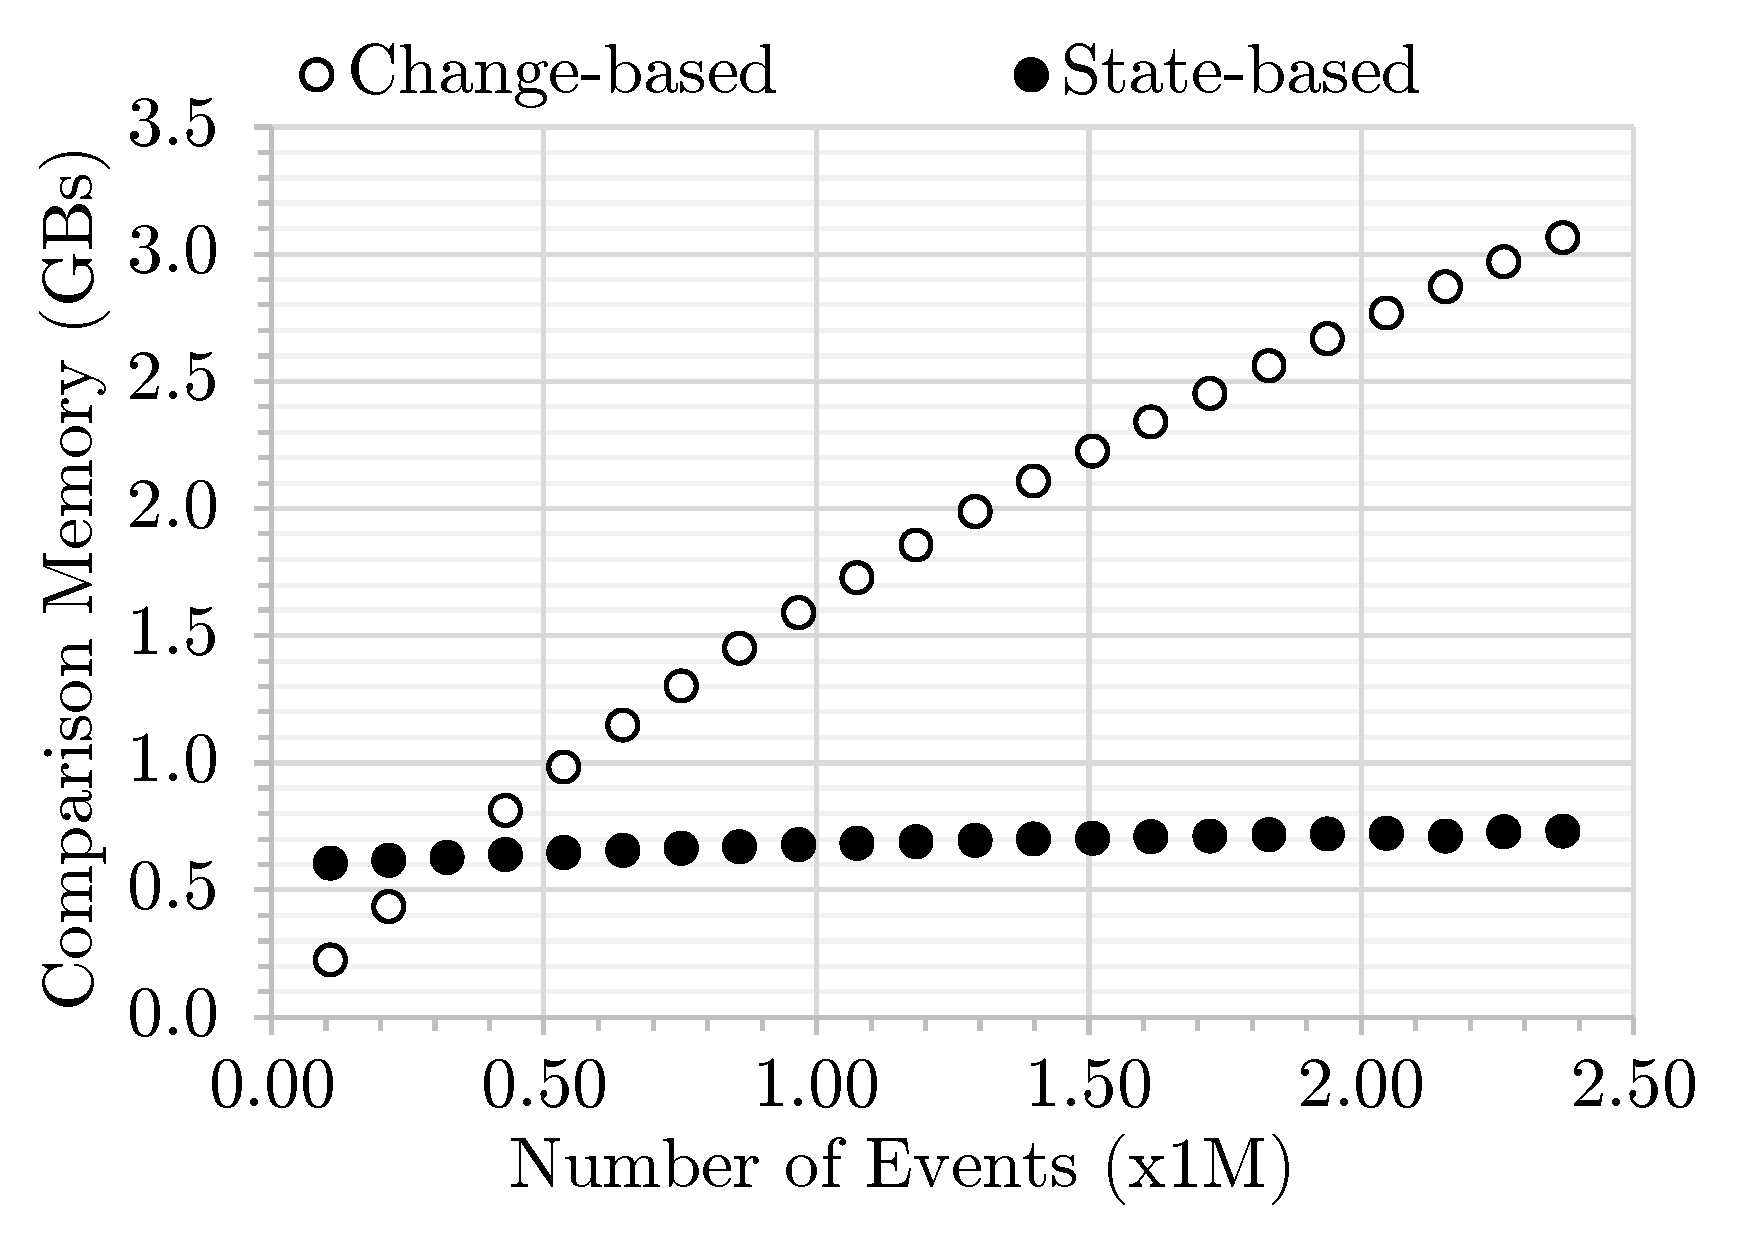
\includegraphics[width=\linewidth]{mixed-memory-events}
    \caption{memory footprint}
    \label{fig:memory_diffs}
  \end{subfigure}
  \caption{Change-based vs. state-based model differencing as differences increase.}
  \label{fig:change_vs_state}
\end{figure}

\vspace{-5pt}
\subsubsection{Mixed Operations}
\label{sec:mixed-operation}

In the mixed operation measurement, we modify two identical models differently by applying random operations. As the number of change events generated by the modification grows, the numbers of affected elements and differences also increase in a logarithmic manner. The patterns can be seen in Figure \ref{fig:modification_course}. The growth is logarithmic since the probability that the random operations modify the same elements also increases. Thus, some change events might not contribute to the addition of new affected elements and differences. In other words, more events are required to increase the number of affected elements or differences. In Figure \ref{fig:modification_course}, the total number of elements remains largely unchanged due to the equal probabilities of addition and deletion as has been set in Section \ref{sec:evaluation}. The figure gives us an insight about the characteristics of the modification caused by the random operations in the mixed operation measurement; it supports explaining the implication of the changes on execution time and memory footprints of model differencing.


\begin{figure}[ht]
    \centering
    \begin{subfigure}[t]{0.495\linewidth}
        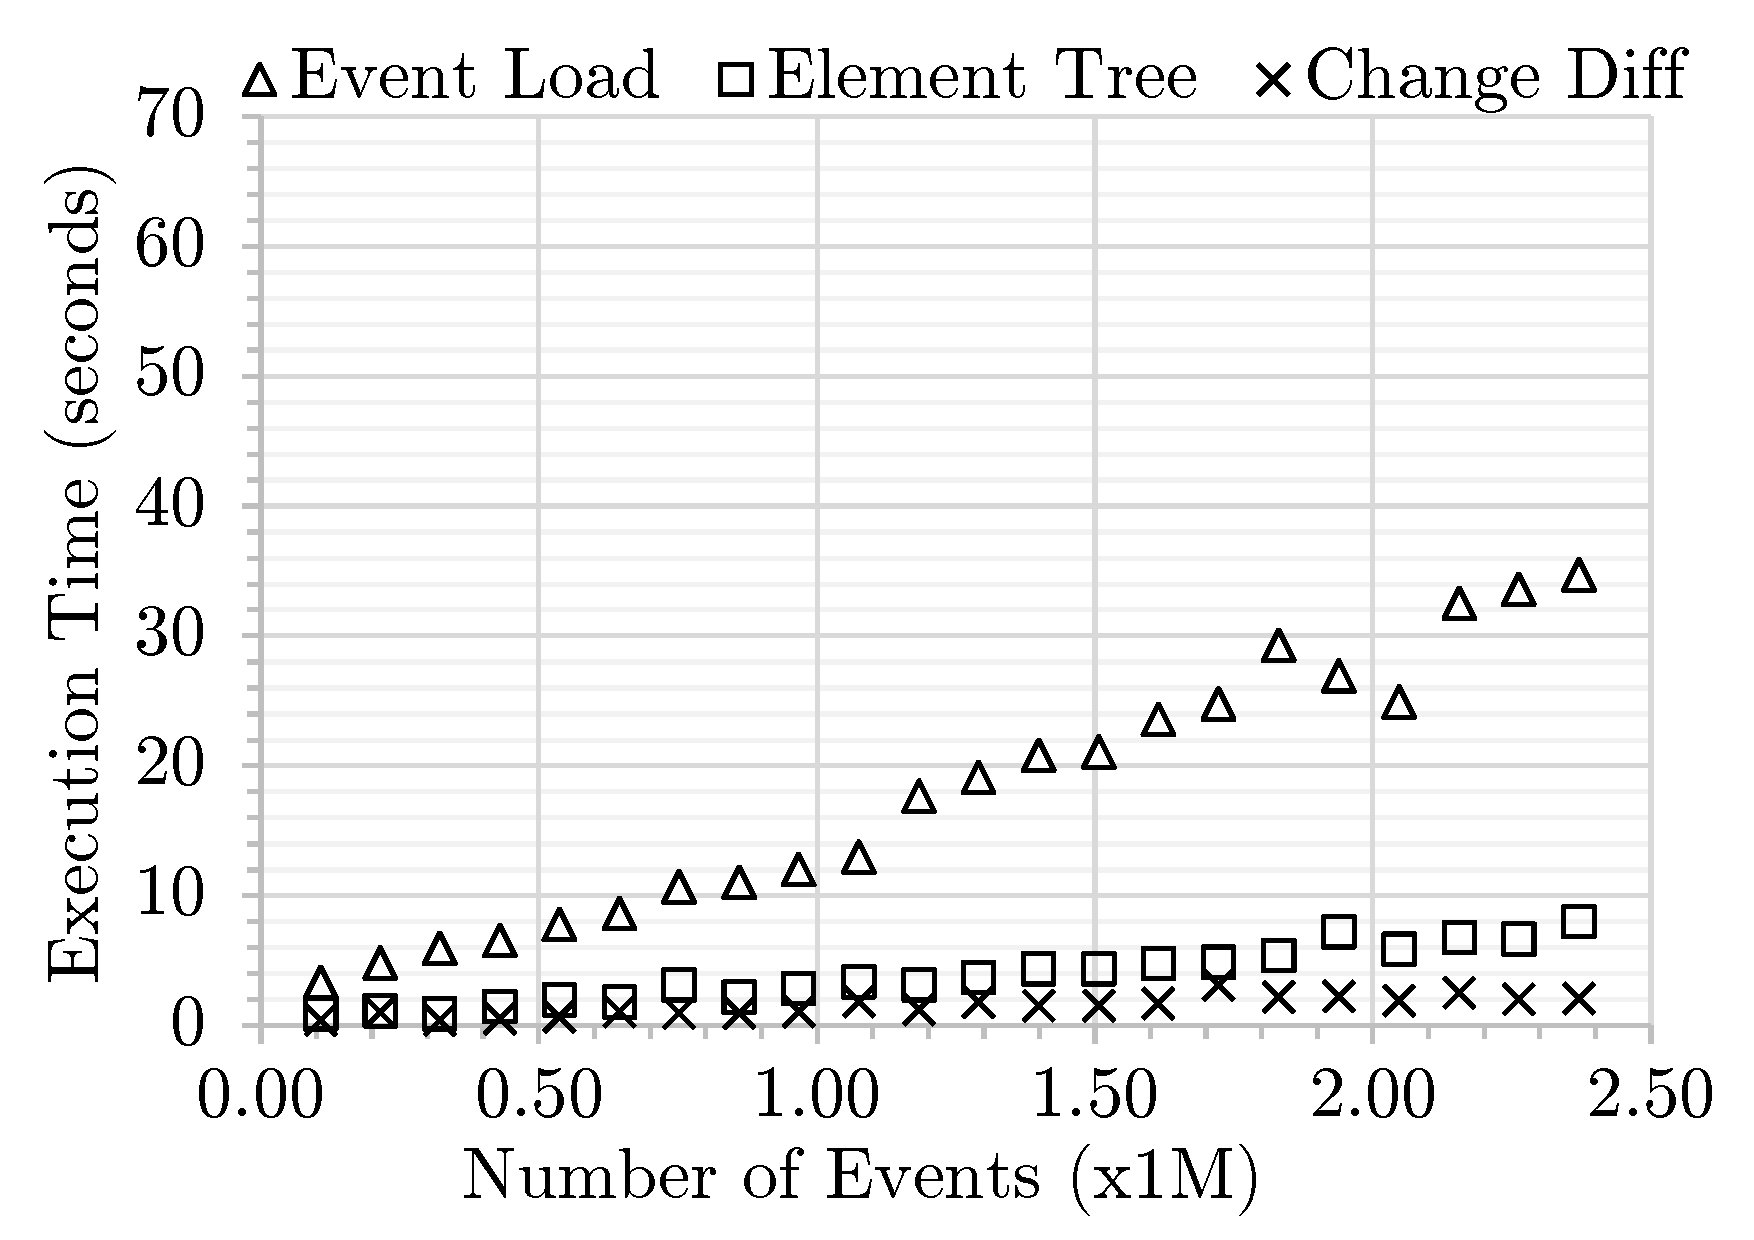
\includegraphics[width=\linewidth]{mixed-time-events-detail}
        \caption{change-based comparison time}
        \label{fig:time_changediff_detail}
    \end{subfigure}
    \hfill
    \begin{subfigure}[t]{0.495\linewidth}
        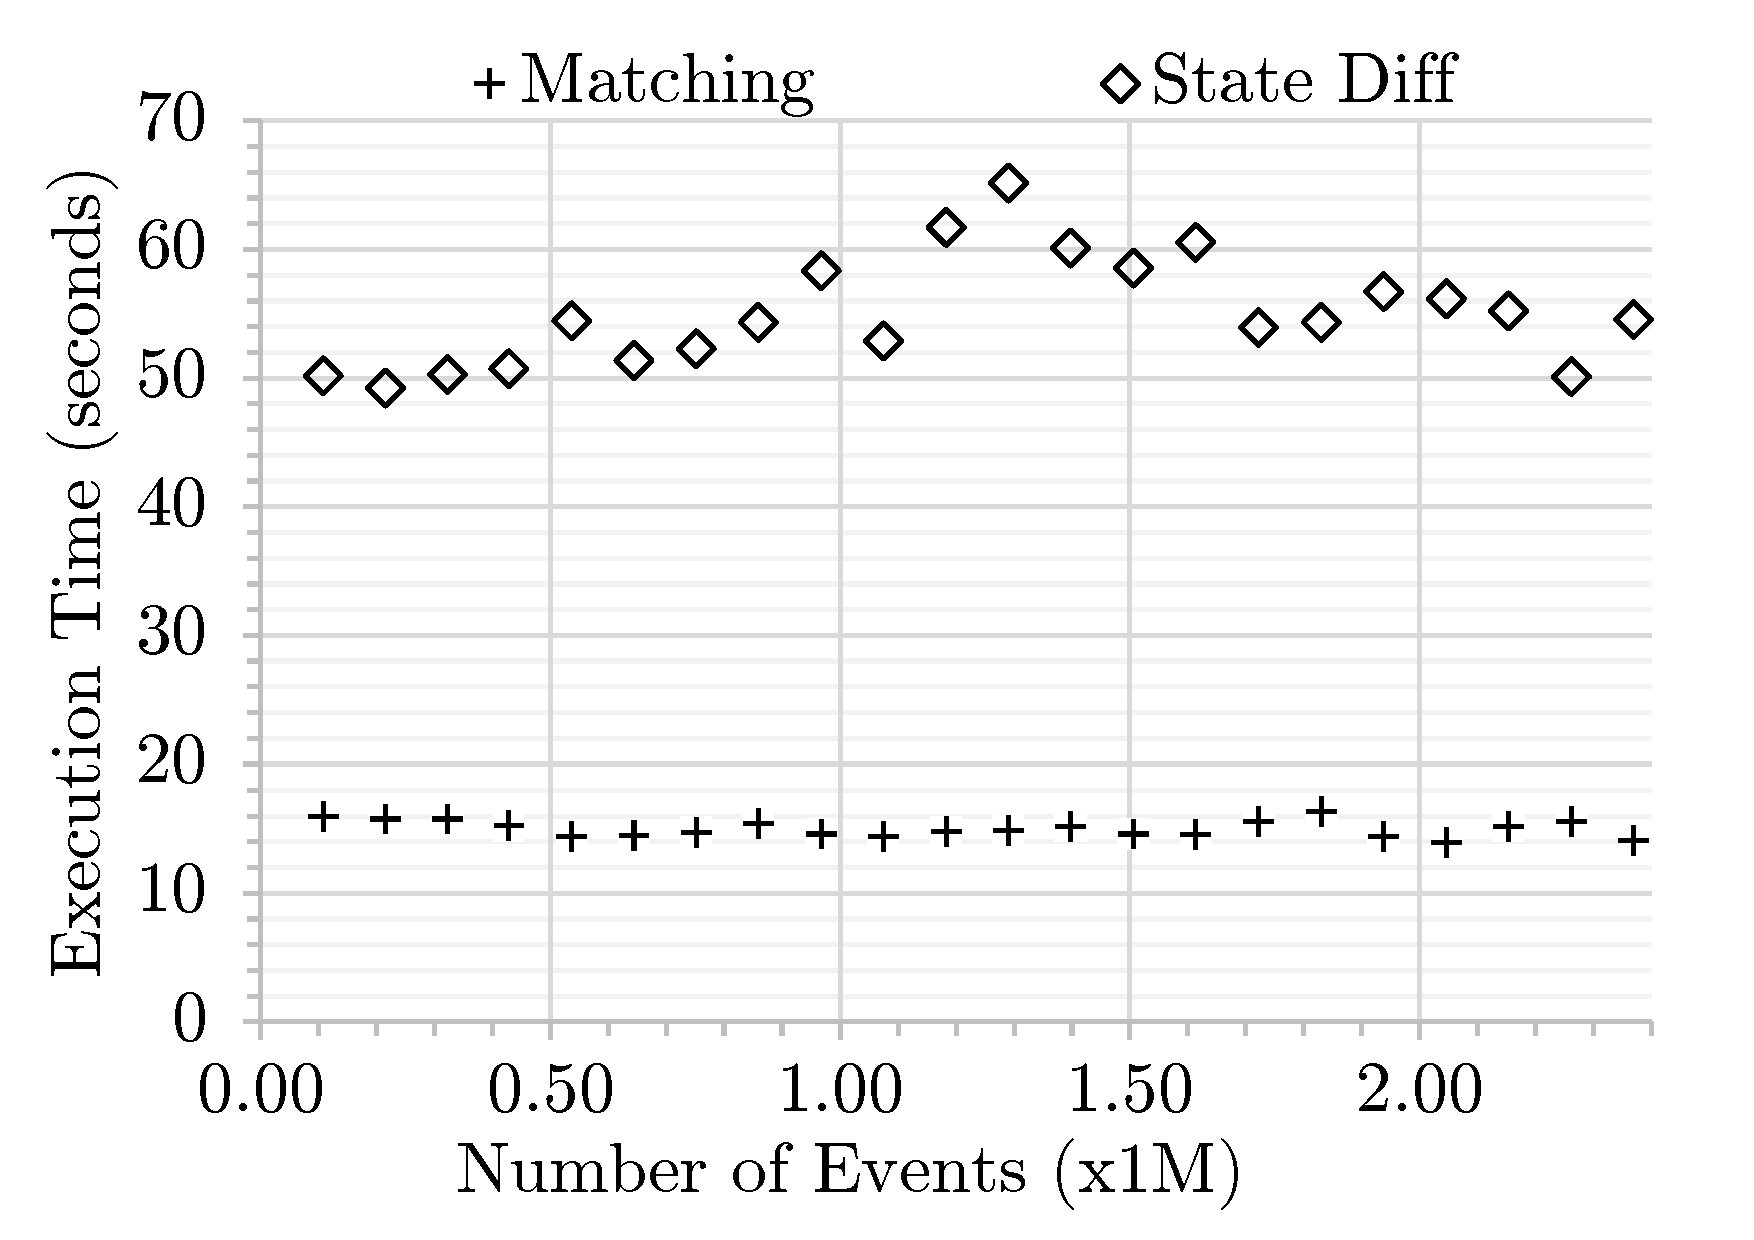
\includegraphics[width=\linewidth]{state-time-events-detail}
        \caption{state-based comparison time}
        \label{fig:time_statediff_detail}
    \end{subfigure}
    \begin{subfigure}[t]{0.495\linewidth}
        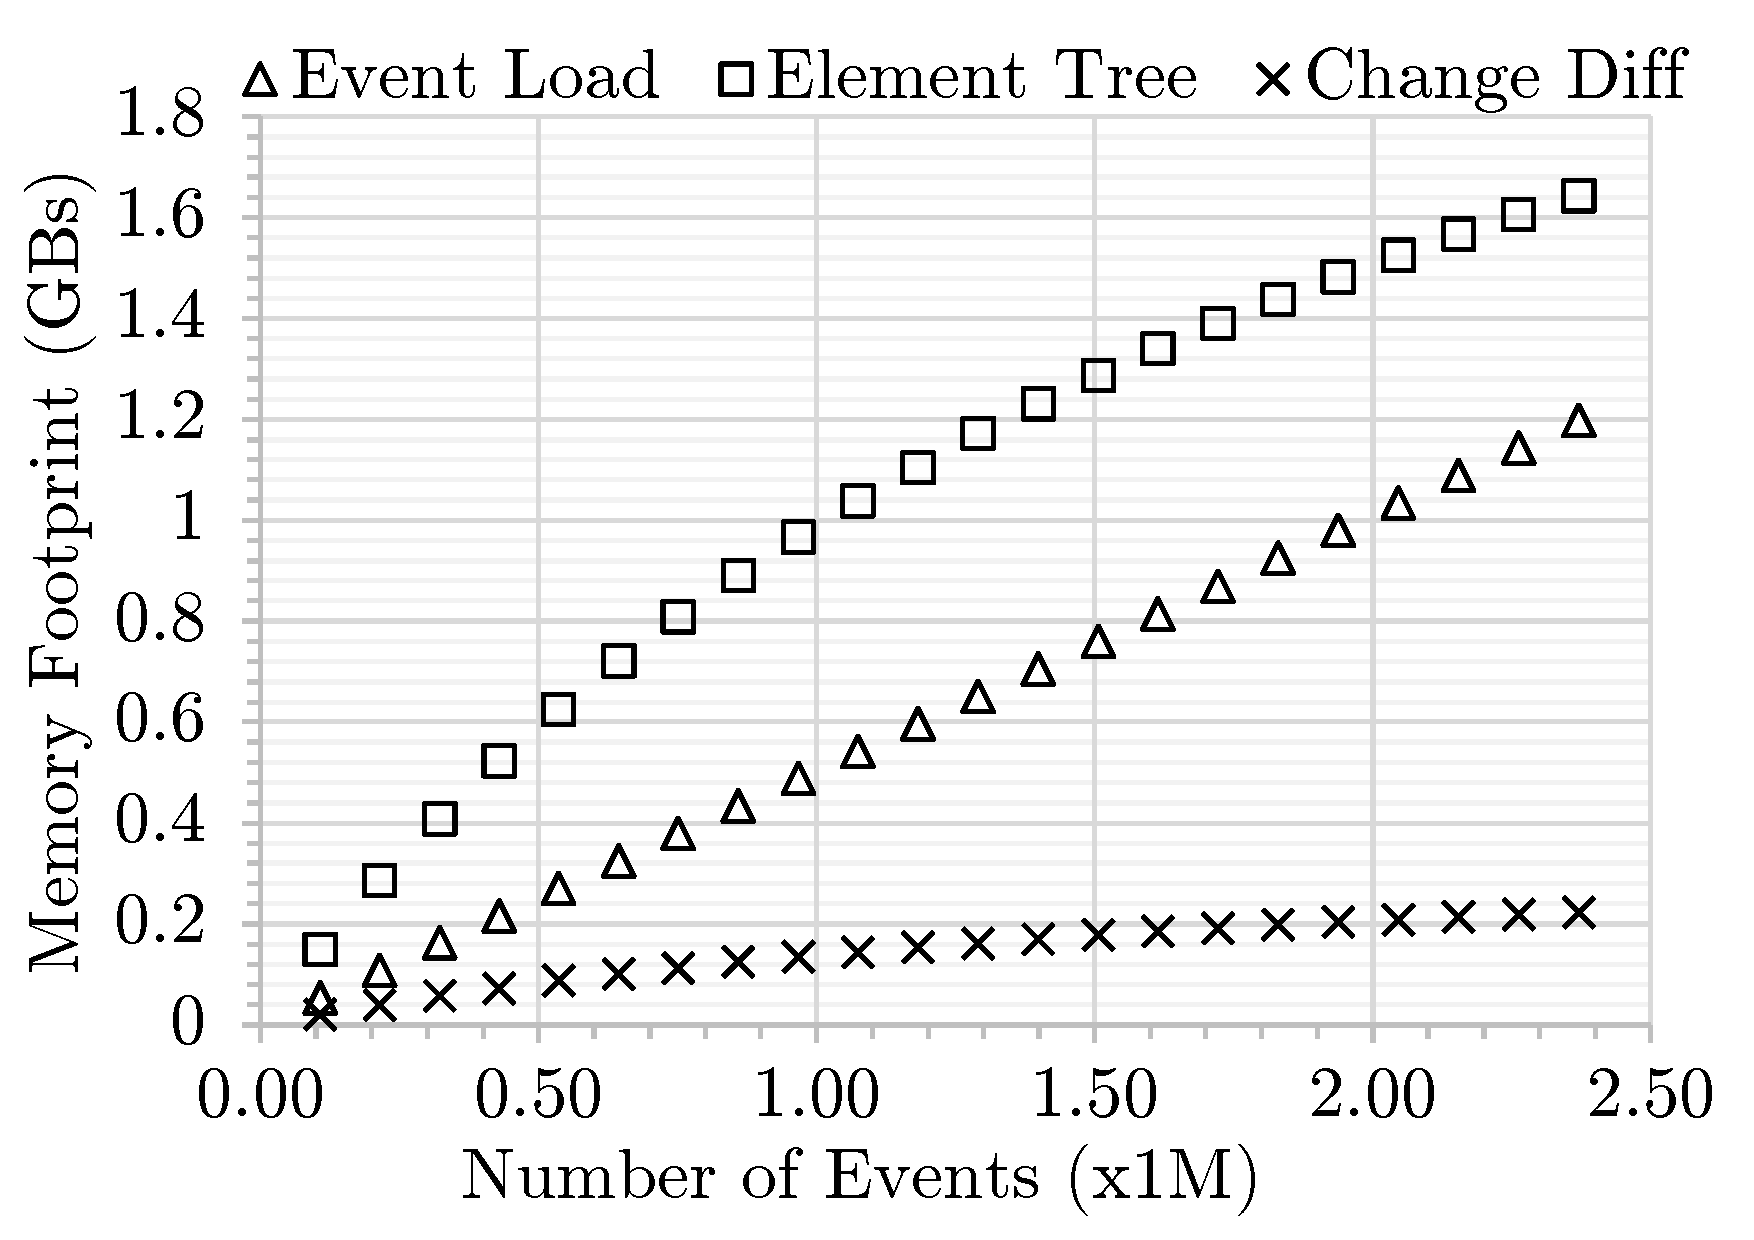
\includegraphics[width=\linewidth]{mixed-memory-events-detail}
        \caption{change-based memory footprint}
        \label{fig:memory_changediff_detail}
    \end{subfigure}
    \hfill
    \begin{subfigure}[t]{0.495\linewidth}
        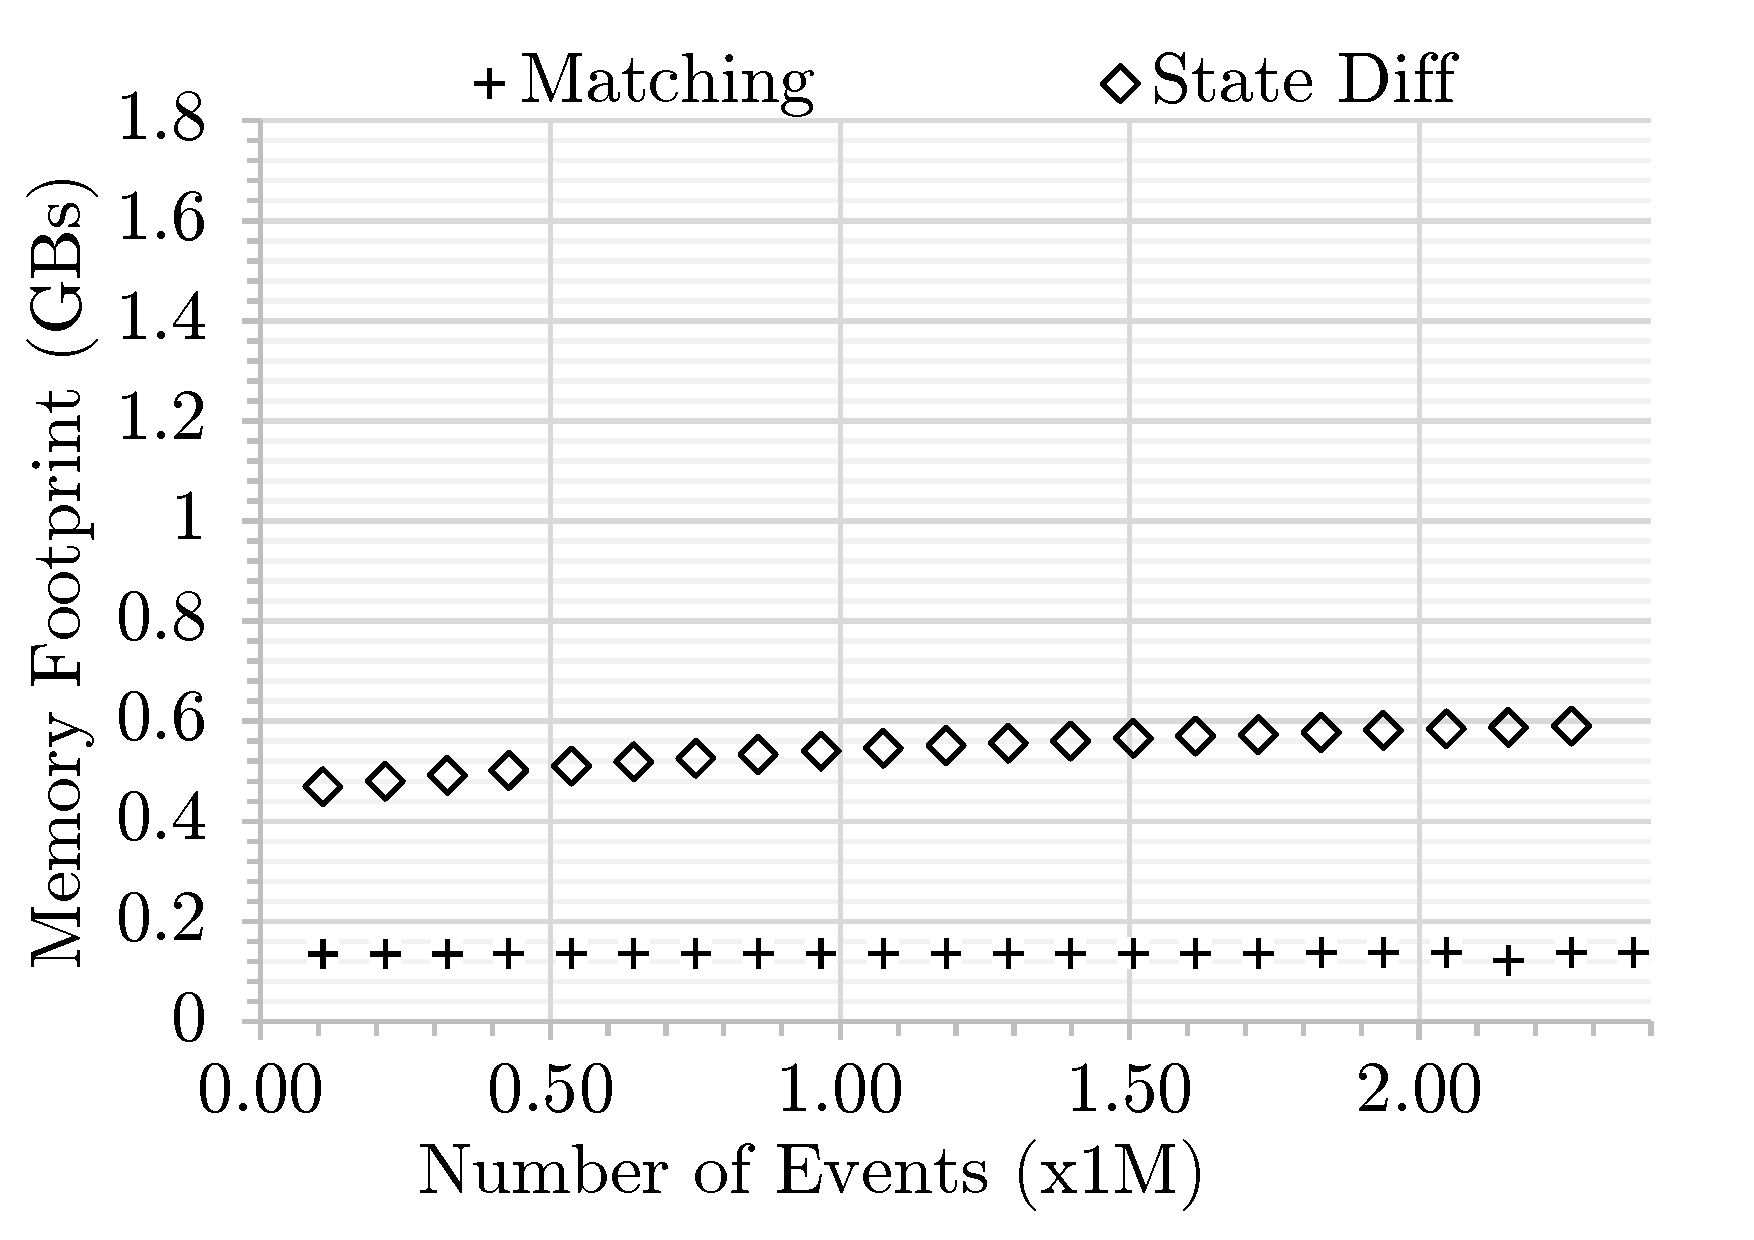
\includegraphics[width=\linewidth]{state-memory-events-detail}
        \caption{state-based memory footprint}
        \label{fig:memory_statediff_detail}
    \end{subfigure}
    \caption{Breakdown view of comparison time and memory footprint in Figure \ref{fig:change_vs_state}.}
    \label{fig:time_memory_detail}
\end{figure}

After applying some random changes on both models, the modification produces 100,000 change events at the first measurement point. Using this amount of events, our change-based comparison only takes 5 seconds to identify around 90,000 differences, in contrast to the state-based comparison that takes 66 seconds (see the first measurement points in Figures \ref{fig:modification_course} and \ref{fig:time_diffs}). If the modification continues, more change events are generated. This growing number of change events has to be loaded into memory and thus slows down the change-based comparison. Nevertheless, the change-based comparison is still faster than the state-based comparison even though the number of change events reaches 2.37 million -- more than 1 million differences at that point; the change-based comparison outperforms the state-based comparison in execution time (Figure \ref{fig:time_diffs}). Figure \ref{fig:time_changediff_detail} breaks down the comparison time in detail. It exhibits that the event loading time is the dominant contributor to the slowdown compared to the element tree's construction time and diffing time. 

For the state-based comparison in Figure \ref{fig:time_statediff_detail}, the comparison time only experiences a slight increase as the number of identified differences also grows.
%\dk{Change to ``grows''?}. 
This slight increase is contributed mainly by the diffing time, while the matching time tends to be constant due to the very small increase of the total elements (Figures \ref{fig:modification_course}).

Nevertheless, change-based comparison generally consumes more memory than the state-based comparison (see Figure \ref{fig:memory_diffs}). It only consumes less memory than its state-based counterpart when the number of events is less than 0.3 million (around less than 0.25 million identified differences at that moment). Figure \ref{fig:memory_changediff_detail} breaks down the memory footprint of change-based comparison into three factors: the loaded change events, element tree, and diffs. As modification continues, an increasing number of events is generated. These events have to be loaded into memory since they contain the required information for the construction of an element tree. The amount of space to keep these change events in memory grows linearly with their number. 

\begin{figure}[ht]
  \centering
  \begin{subfigure}[t]{0.495\linewidth}
    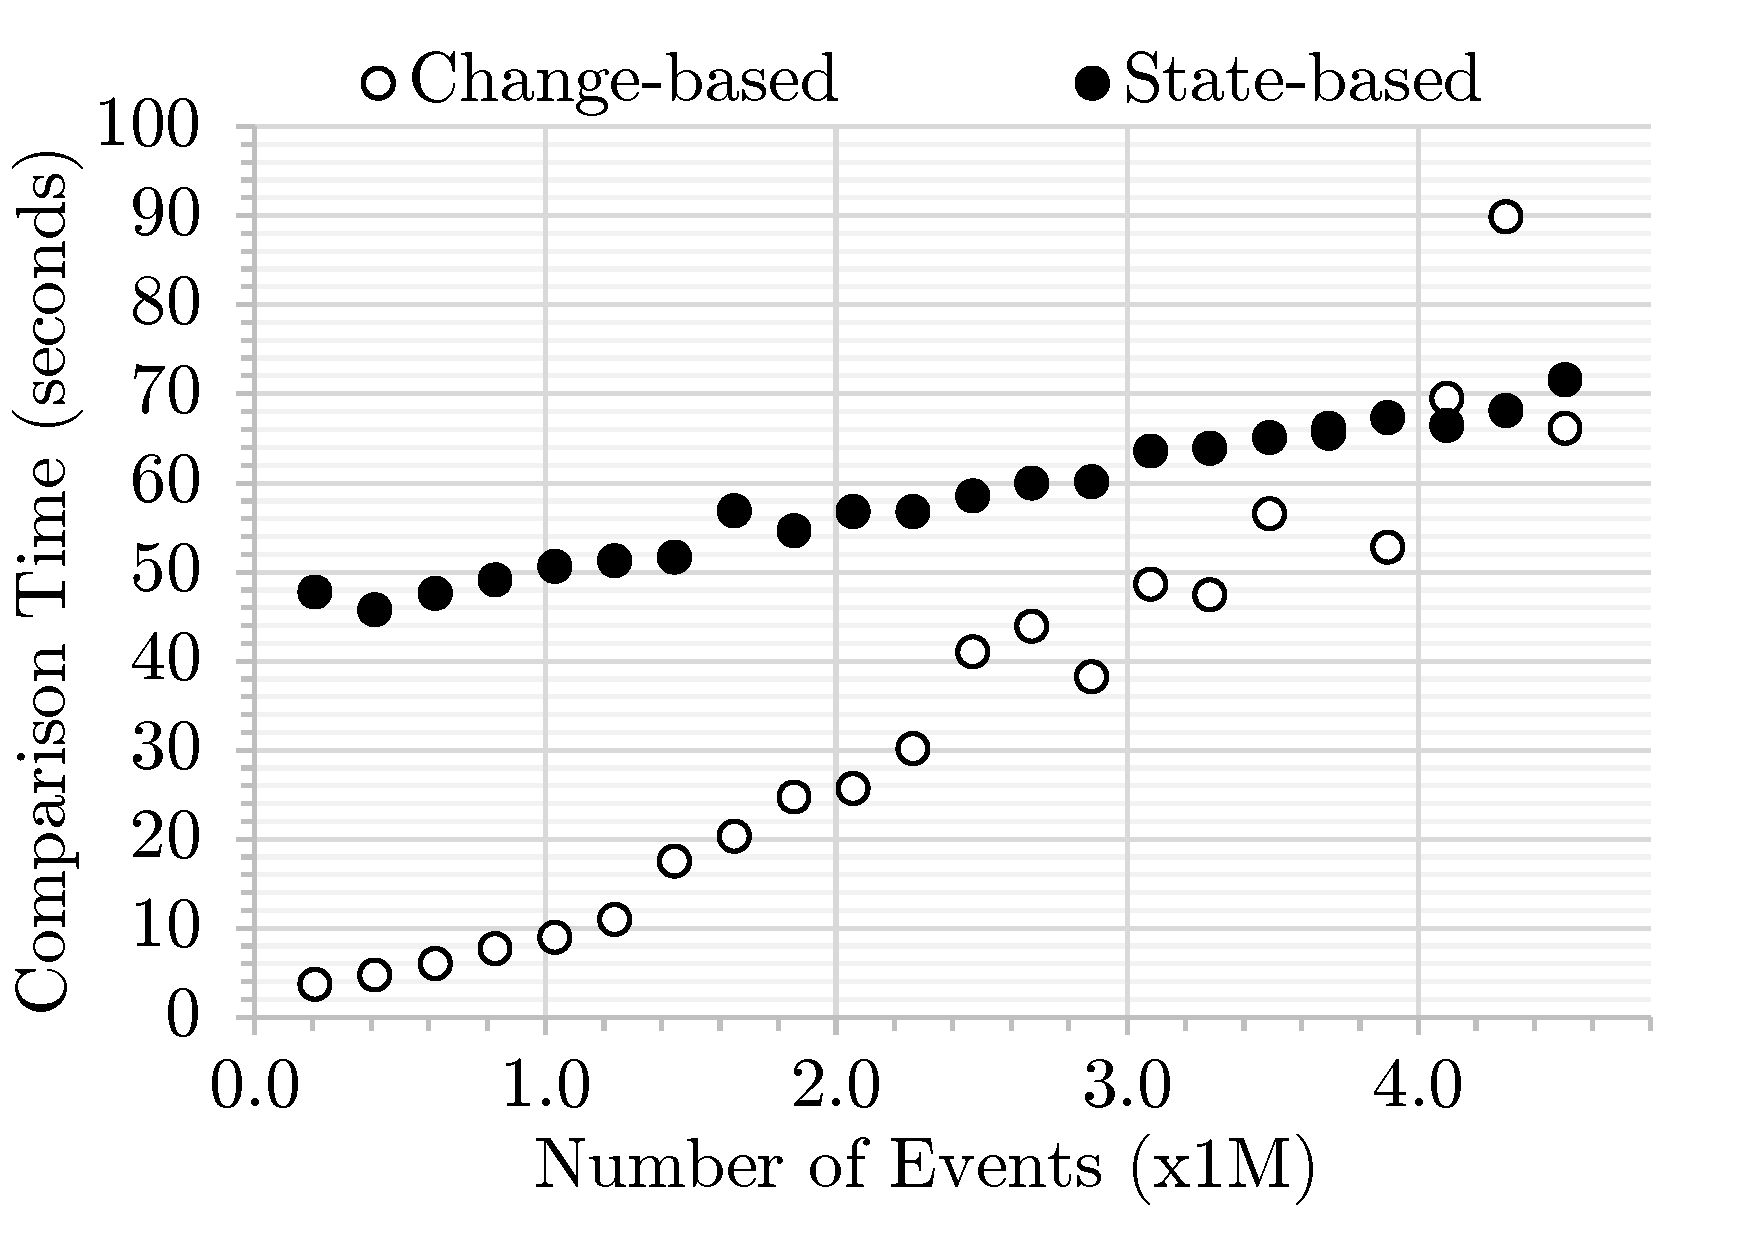
\includegraphics[width=\linewidth]{add-time-events}
    \caption{add-only}
    \label{fig:add-time-events}
  \end{subfigure}
  \hfill
  \begin{subfigure}[t]{0.495\linewidth}
    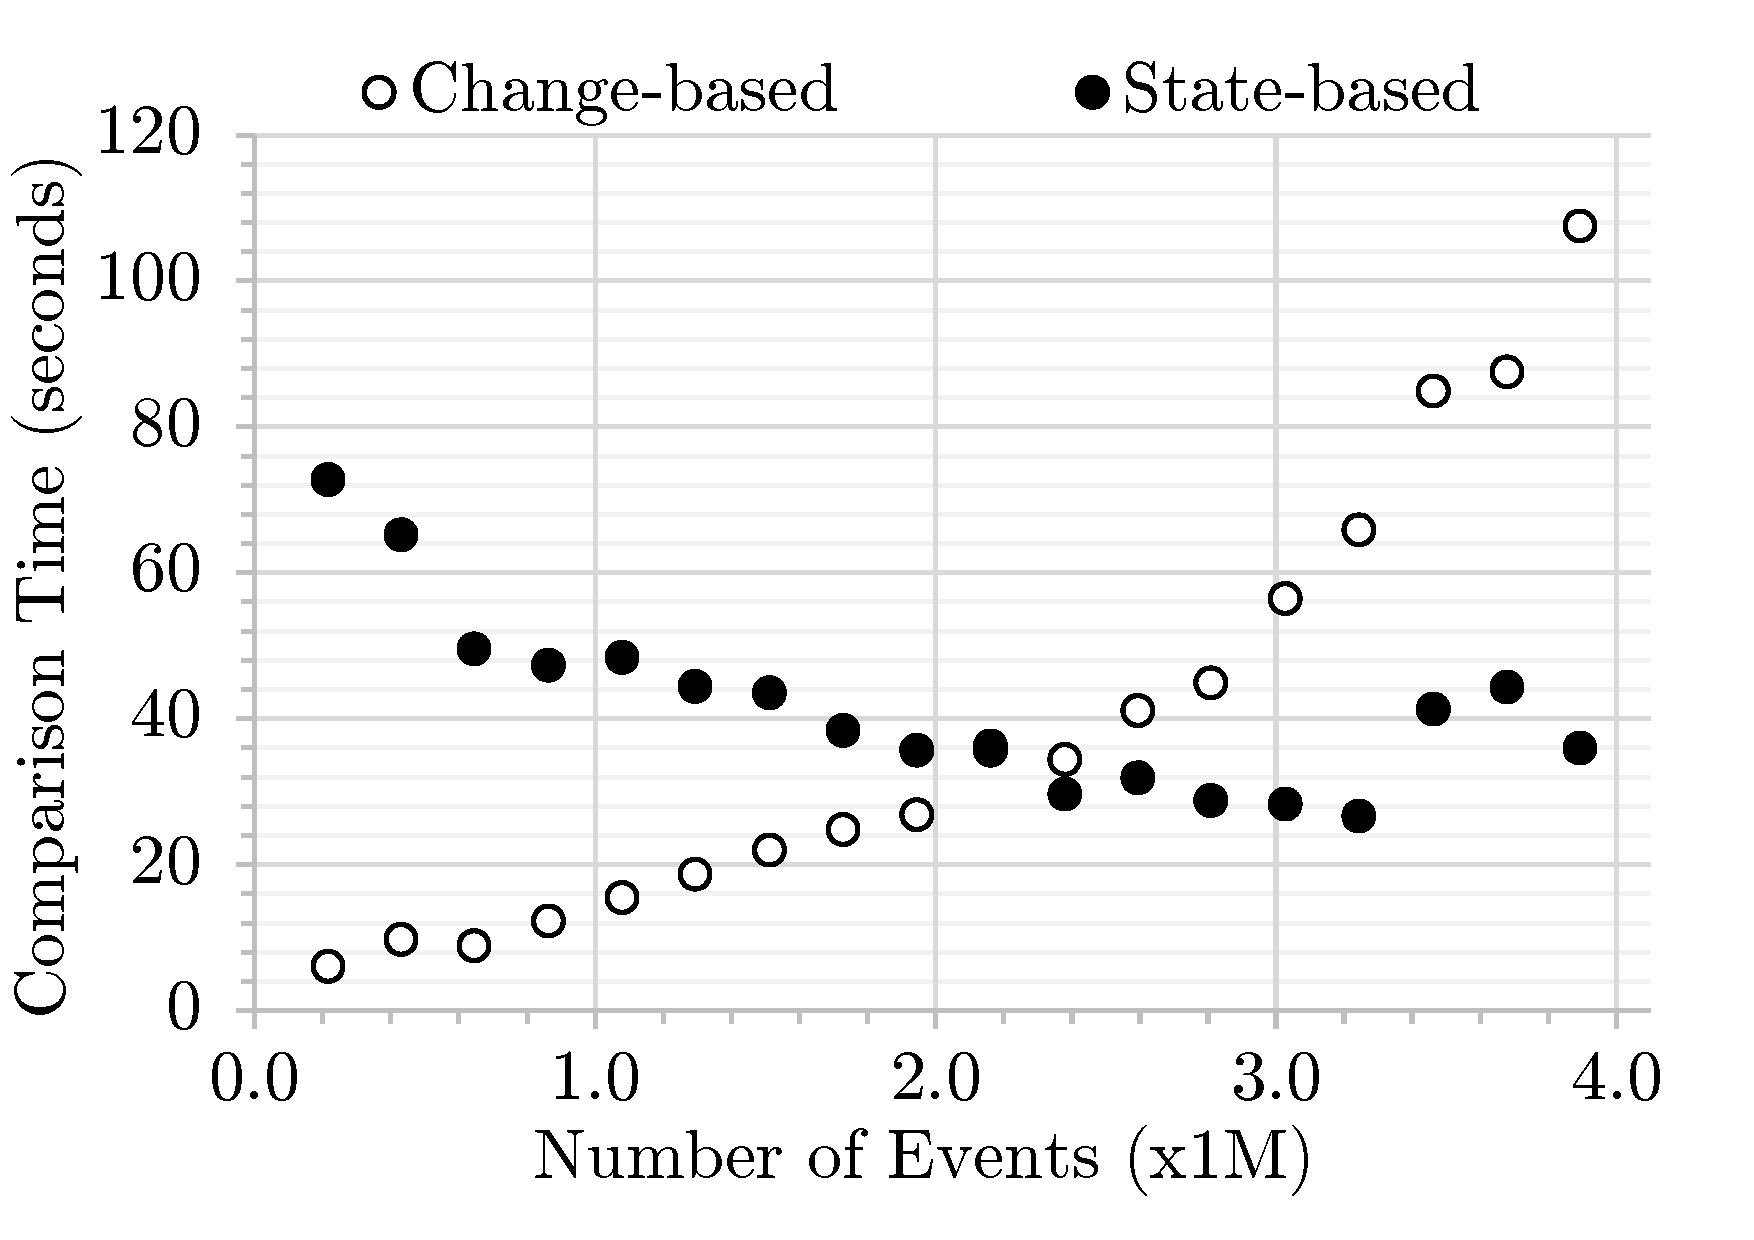
\includegraphics[width=\linewidth]{delete-time-events}
    \caption{delete-only}
    \label{fig:delete-time-events}
  \end{subfigure}
  \begin{subfigure}[t]{0.495\linewidth}
    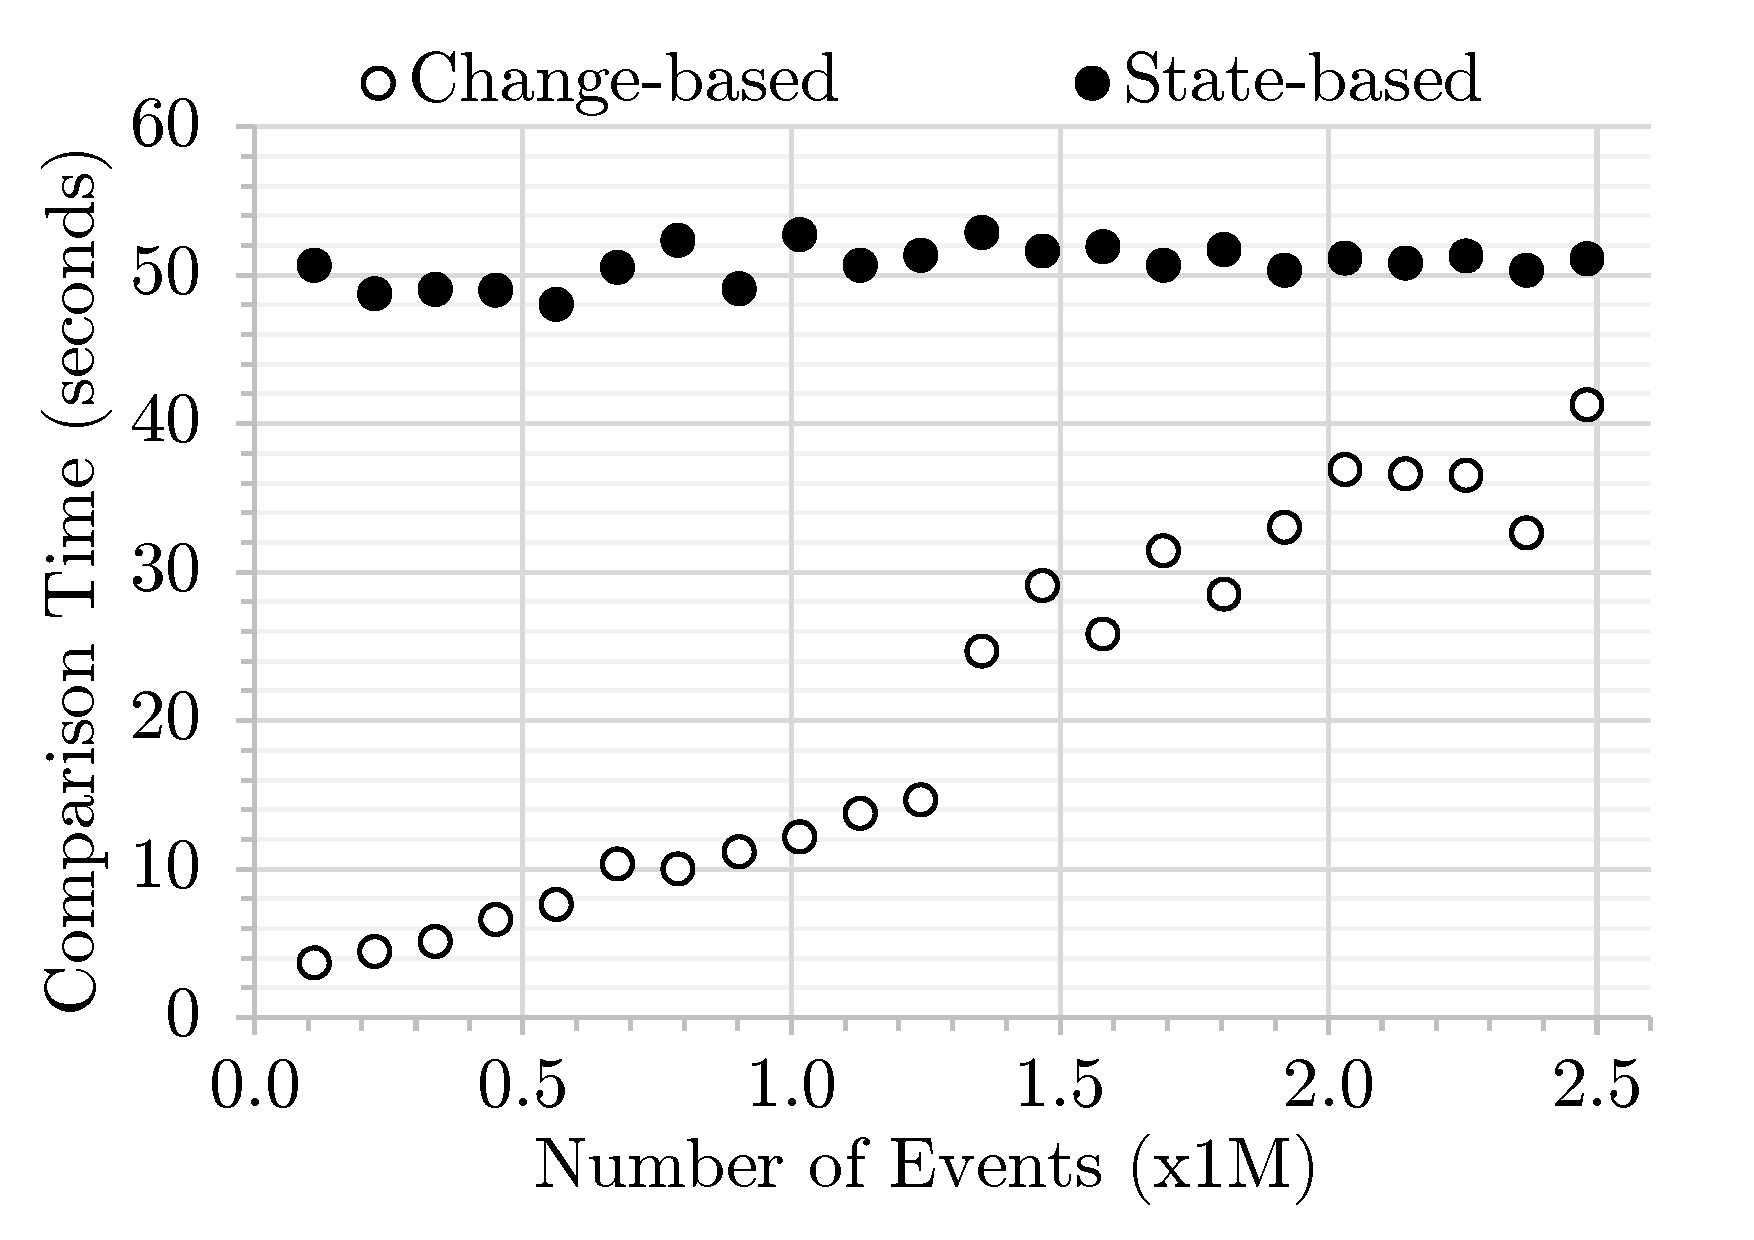
\includegraphics[width=\linewidth]{move-time-events}
    \caption{move-only}
    \label{fig:move-time-events}
  \end{subfigure}
  \hfill
  \begin{subfigure}[t]{0.495\linewidth}
    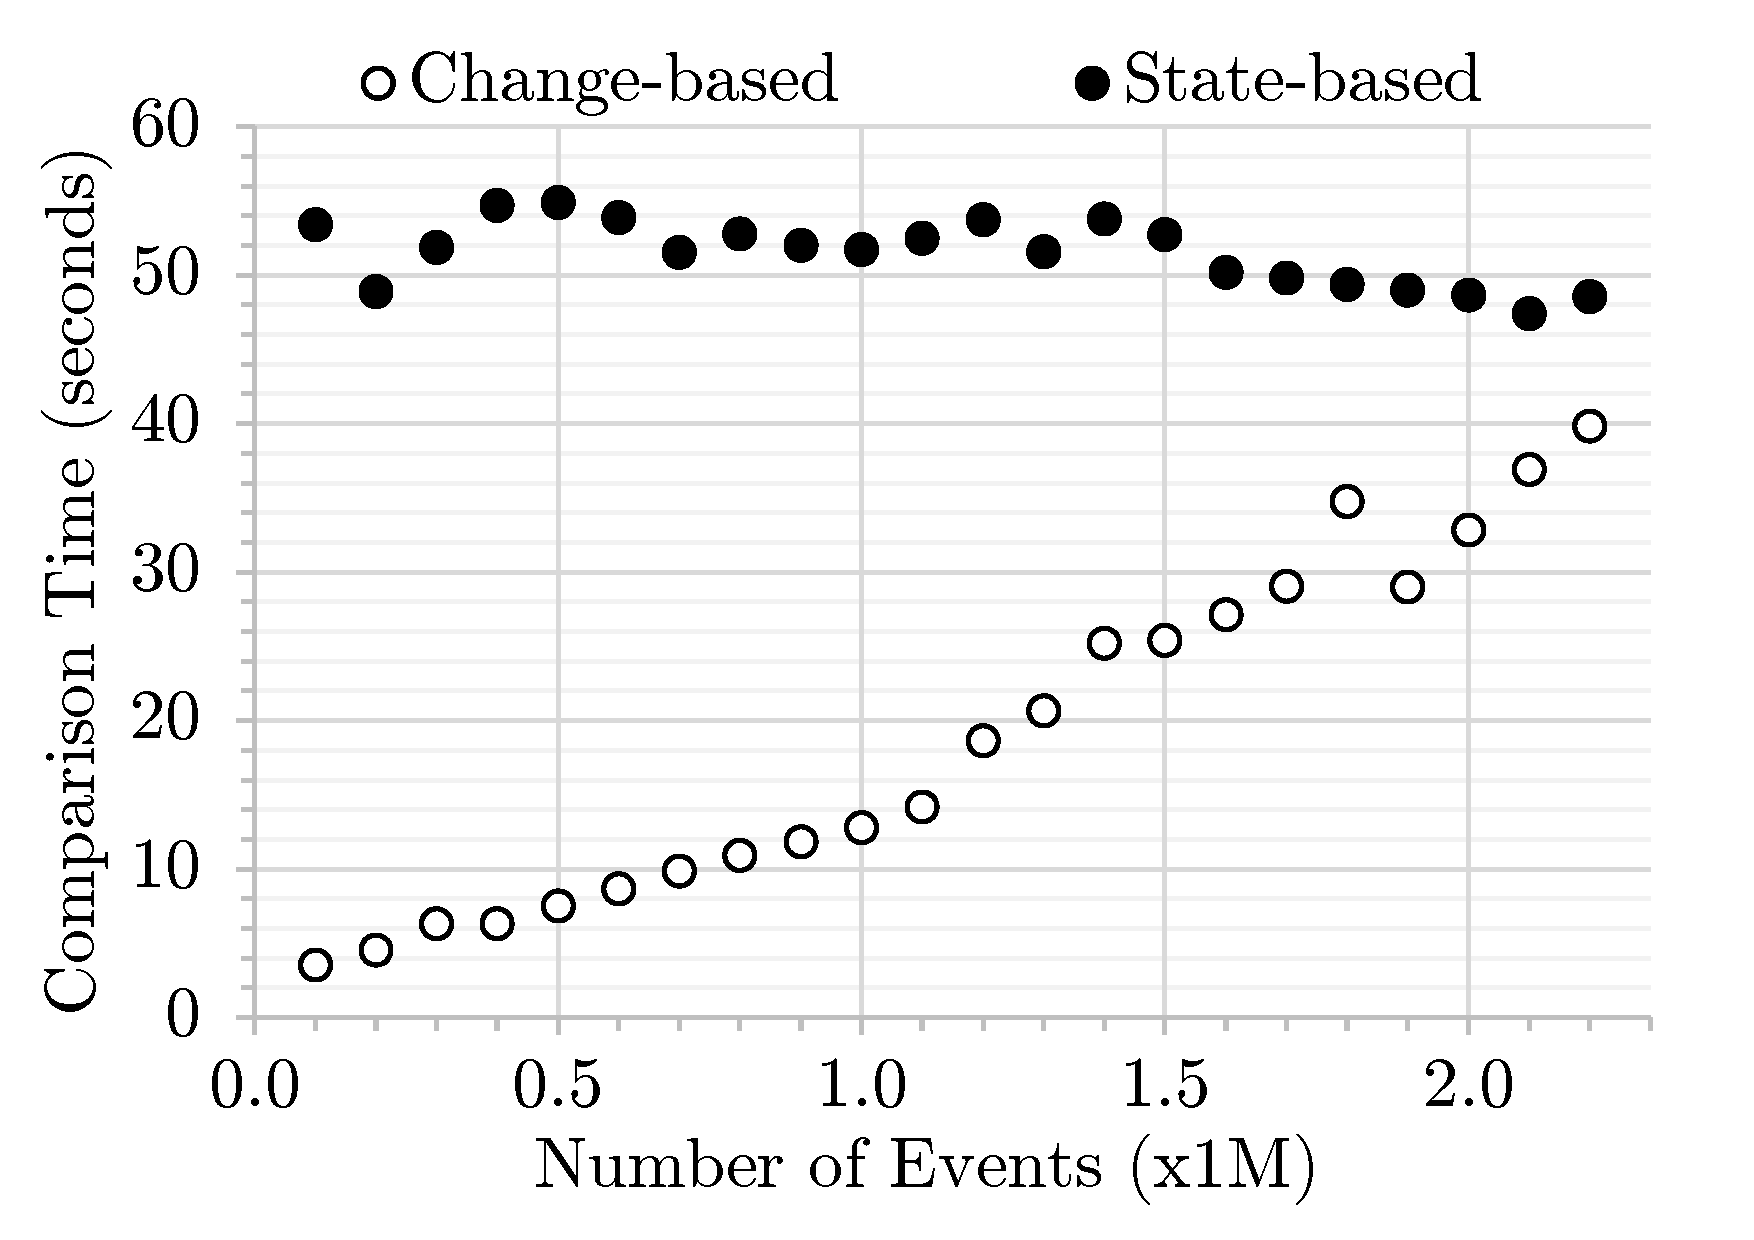
\includegraphics[width=\linewidth]{change-time-events}
    \caption{change-only}
    \label{fig:change-time-events}
  \end{subfigure}
  \caption{Comparison time for homogeneous operations.}
  \label{fig:operation_time_events}
\end{figure}

In contrast, the memory used for the element tree grows logarithmically. As the number of events increases, the probability that events modify already affected elements also increases. Thus, no additional memory allocation is required for the element tree. We can also notice that the element tree occupies most of the memory footprint since it mirrors the partial states -- elements, features, and values -- of the models that are affected by the changes. Moreover, in our technical implementation, a feature can have many instances -- one instance for each element (As a comparison, in the EMF implementation, there is only one instance for a feature. The feature is used as a key so that different elements can have the same feature that maps to different values simultaneously). This contributes to the large memory footprint used by the element tree. The identified change-based diffs, the third factor, are the smallest factor that contributes to the memory footprint of the change-based comparison. 

For the state-based comparison in Figure \ref{fig:memory_statediff_detail}, the memory footprint only grows slightly along the increase of differences. A large part of the memory footprint is used to represent the identified differences, while the memory used for matches tends to be constant as the changes of the total elements are very small -- less new elements means less memory needs to be allocated for new matches (Figures \ref{fig:modification_course}). 

\subsubsection{Homogeneous Operations}
\label{sec:homogeneous-operation}



\begin{figure}[ht]
    \centering
    \begin{subfigure}[t]{0.495\linewidth}
        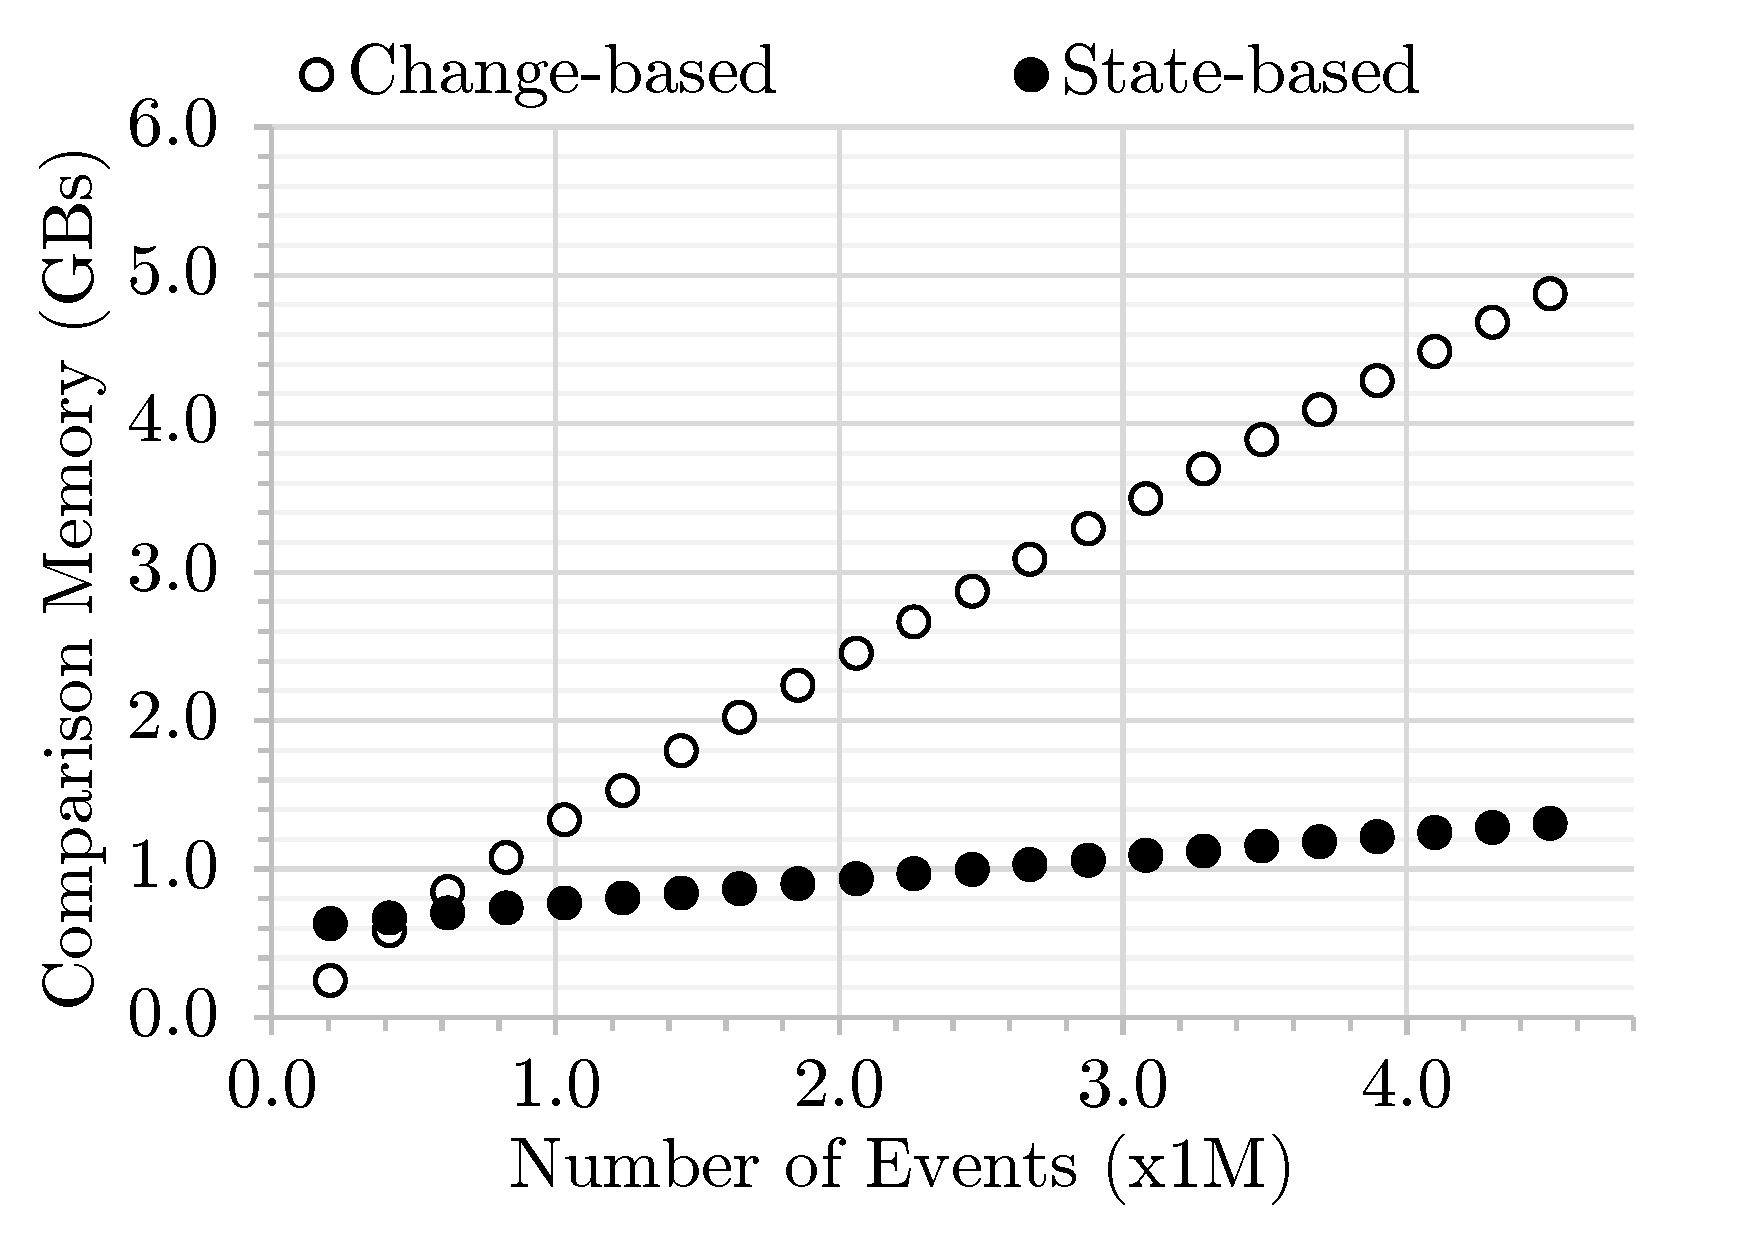
\includegraphics[width=\linewidth]{add-memory-events}
        \caption{add-only}
        \label{fig:add-memory-events}
    \end{subfigure}
    \hfill
    \begin{subfigure}[t]{0.495\linewidth}
        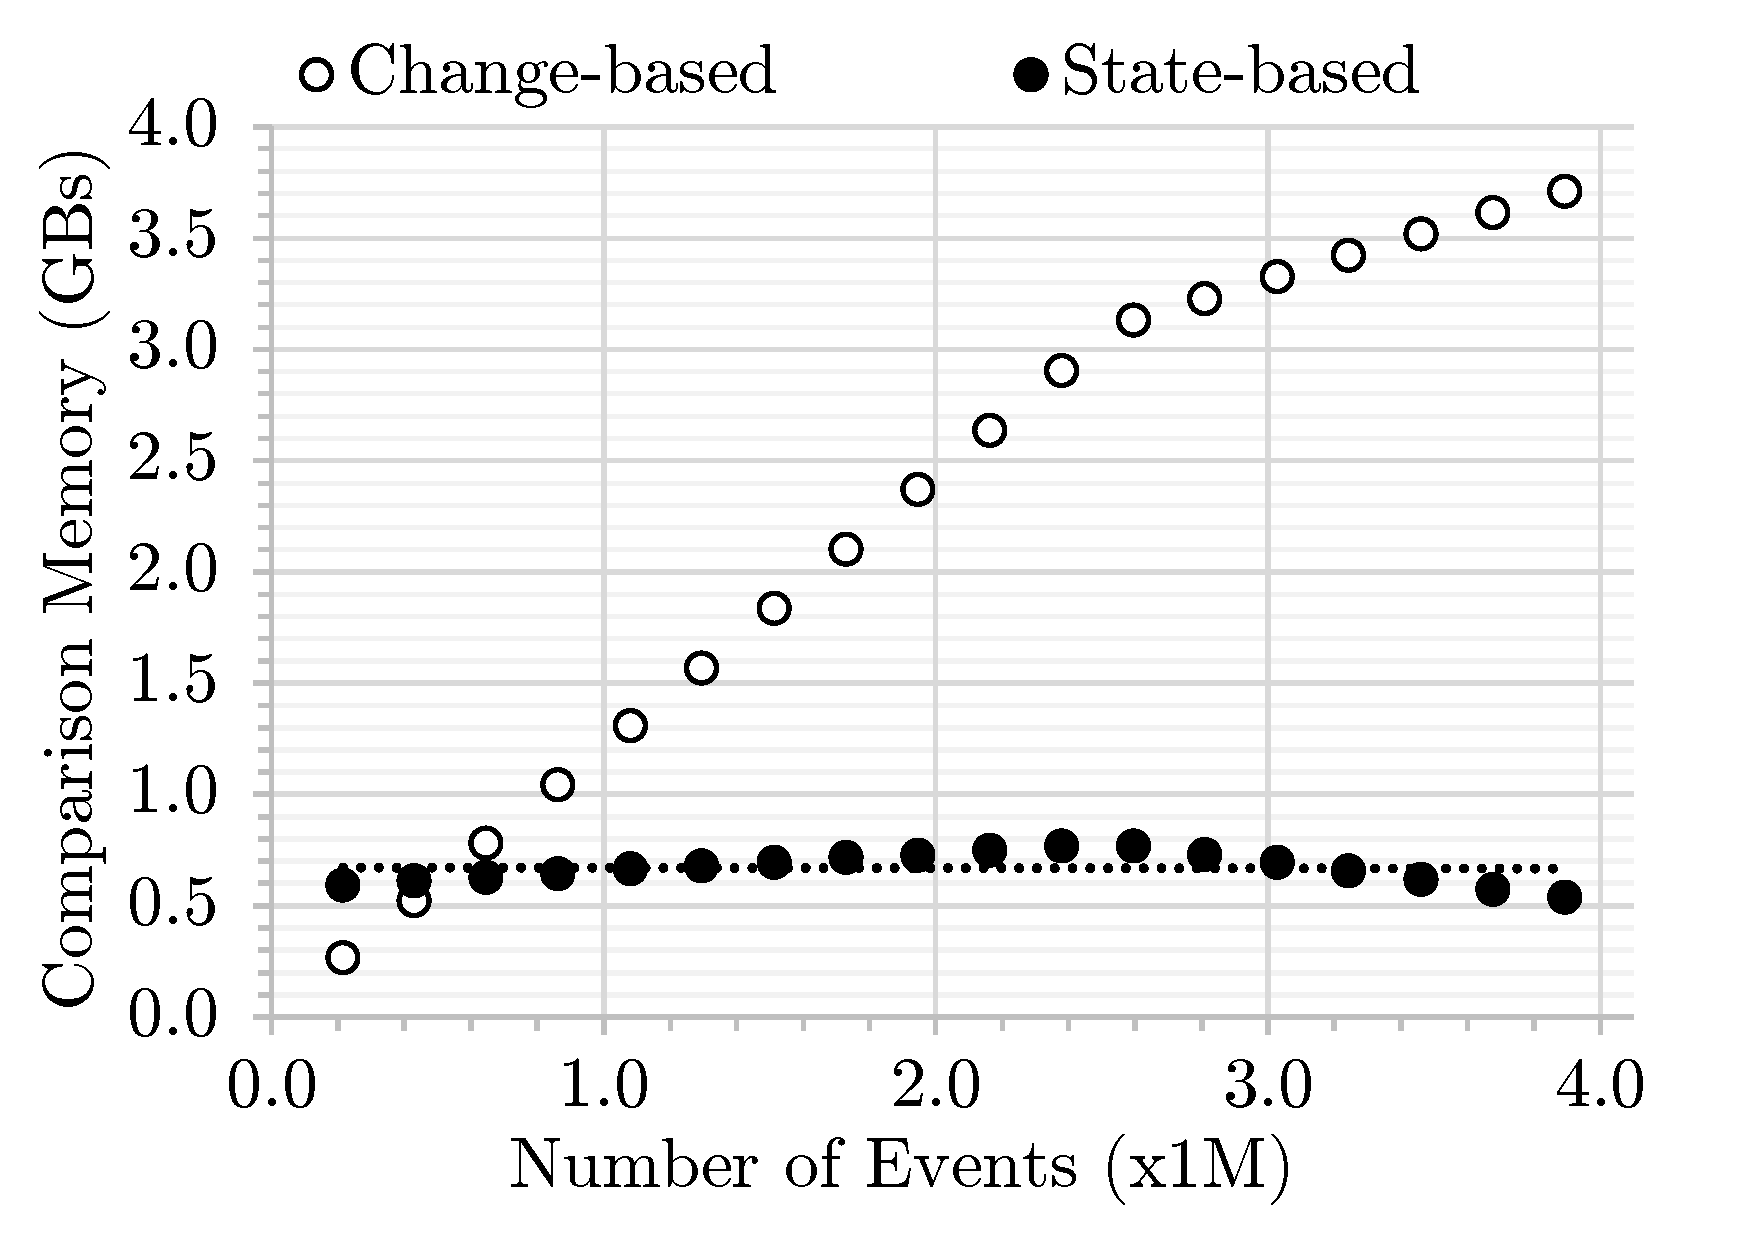
\includegraphics[width=\linewidth]{delete-memory-events}
        \caption{delete-only}
        \label{fig:delete-memory-events}
    \end{subfigure}
    \begin{subfigure}[t]{0.495\linewidth}
        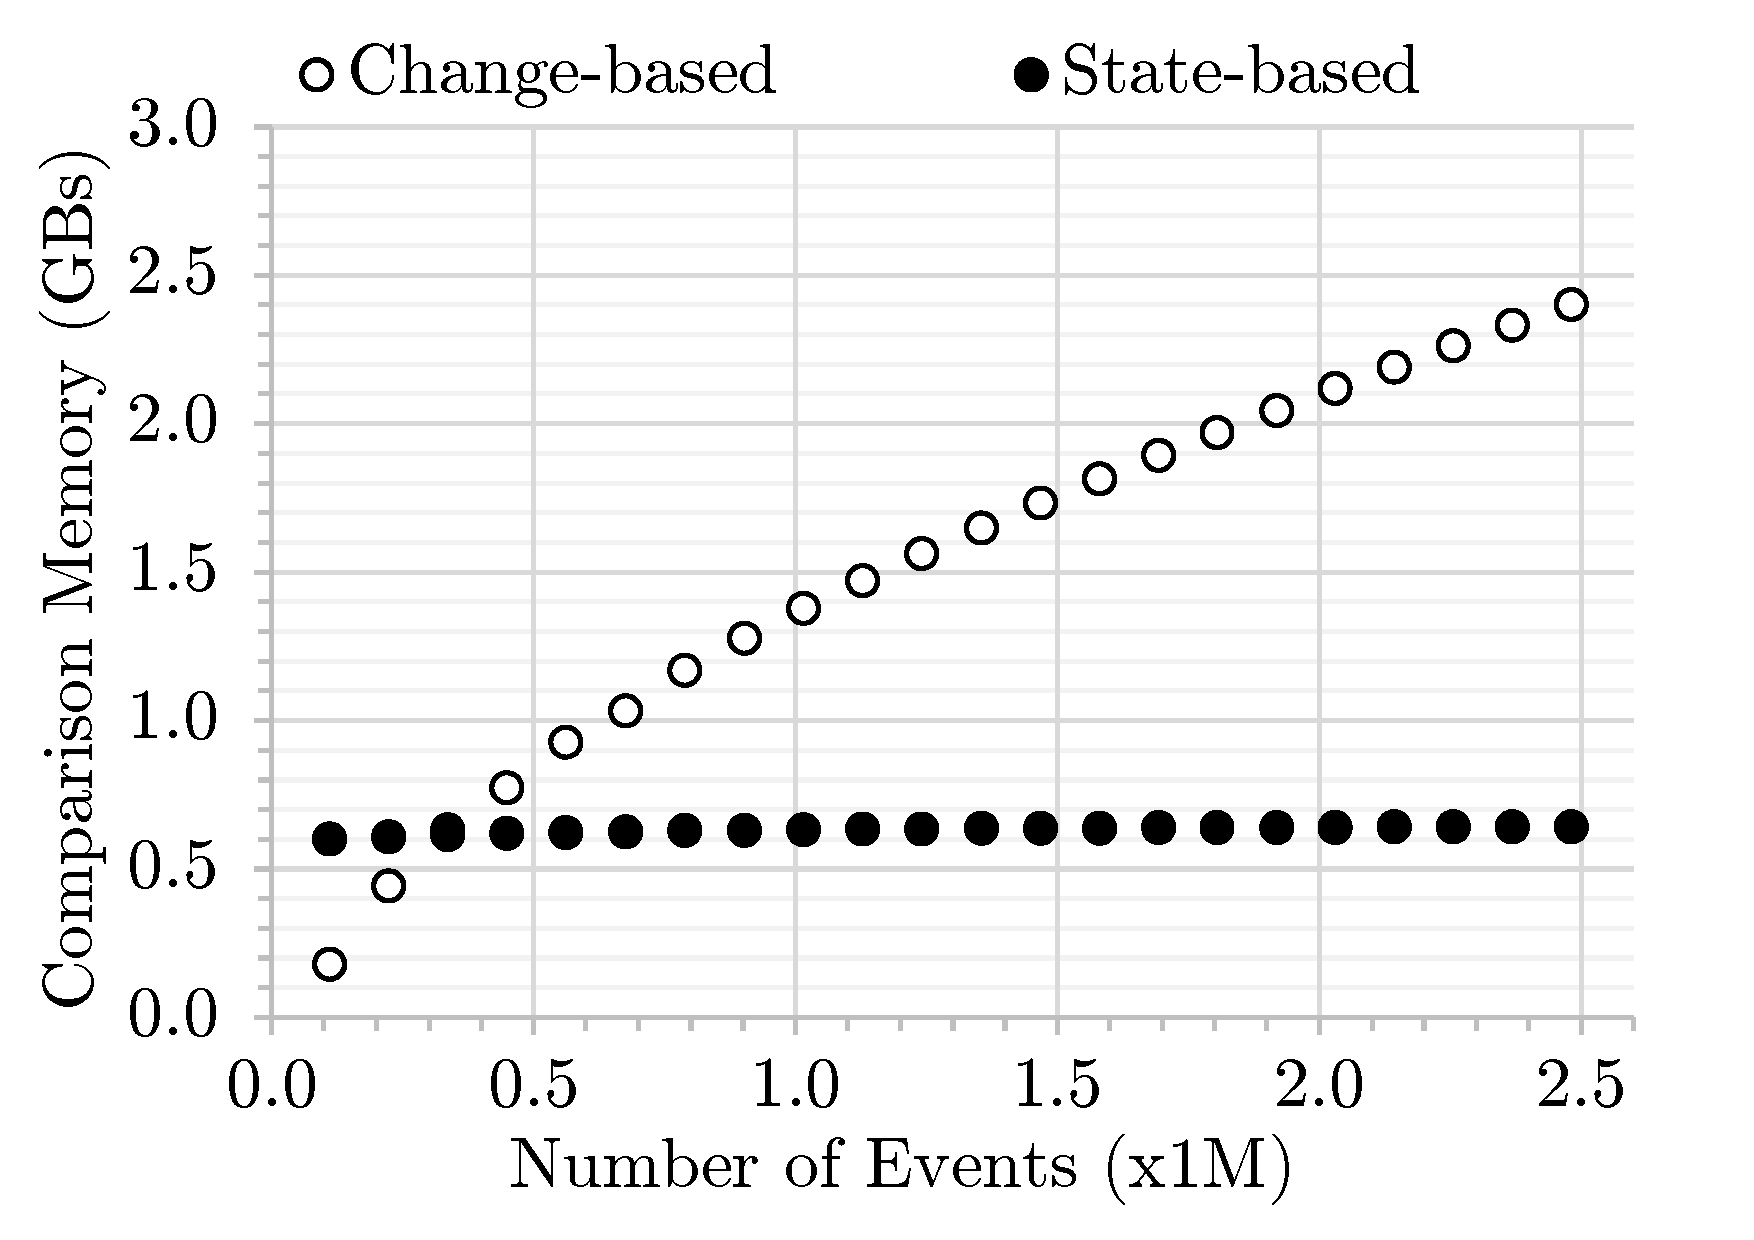
\includegraphics[width=\linewidth]{move-memory-events}
        \caption{move-only}
        \label{fig:move-memory-events}
    \end{subfigure}
    \hfill
    \begin{subfigure}[t]{0.495\linewidth}
        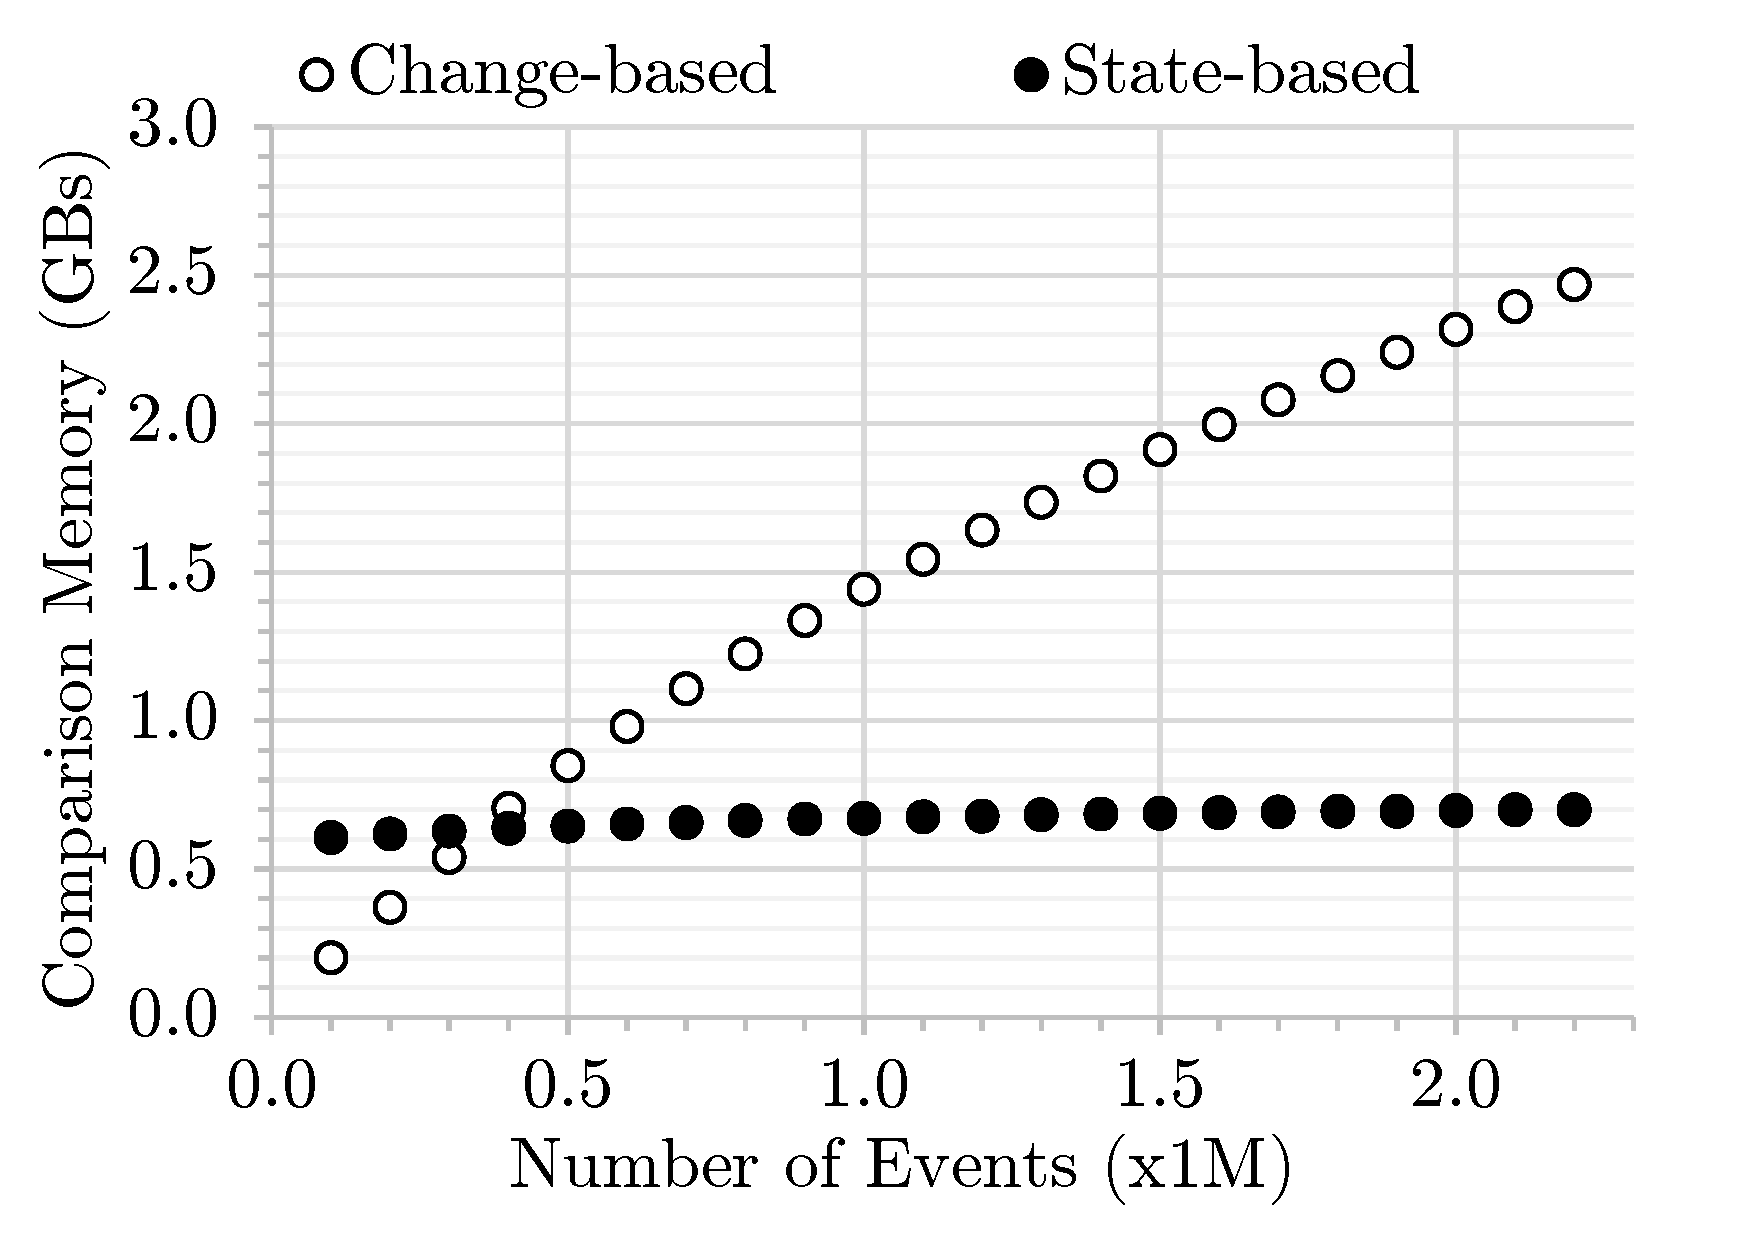
\includegraphics[width=\linewidth]{change-memory-events}
        \caption{change-only}
        \label{fig:change-memory-events}
    \end{subfigure}
    \caption{Memory footprint for homogeneous operations.}
    \label{fig:operation_memory_events}
\end{figure}

Figures \ref{fig:operation_time_events} and \ref{fig:operation_memory_events} exhibit the comparison time and memory footprint of models that have been modified using homogeneous operations -- \textsf{add}, \textsf{remove}, \textsf{move}, or \textsf{set} only. We can notice that in all figures change-based comparison outperforms its state-based counterpart, particularly when the number of change events is small relative to the size of the model. As the number of modifications grows, eventually change-based comparison becomes slower than state-based comparison. In our experiments, this happens when the number of events is greater than 4 million (Figure \ref{fig:add-time-events}). Change-based comparison also becomes slower when the size of models shrinks (due to a large number of delete events) as depicted in Figure \ref{fig:delete-memory-events} as the change-based comparison still needs to load these change events and construct its element tree; in contrast, deletion means less work for state-based comparison. In terms of memory footprint, change-based comparison only performs better than state-based comparison when the number of change events is less than 0.3 millions as depicted in Figure \ref{fig:operation_memory_events}.

\section{Conclusions}
\label{sec:conclusions_6}

Based on the findings, we argue that the change-based comparison approach works at its best for large models that have been modified a moderate number of times. Models that have been excessively modified and experience significant reduction on model size could impair the performance of change-based comparison as a great number of change records have to be read and loaded into memory. 
